%%%%%%%%%%%%%%%%%%%%%%%%%%%%%%%%%%%%%%%%%
% Arsclassica Article
% LaTeX Template
% Version 1.1 (1/8/17)
%
% This template has been downloaded from:
% http://www.LaTeXTemplates.com
%
% Original author:
% Lorenzo Pantieri (http://www.lorenzopantieri.net) with extensive modifications by:
% Vel (vel@latextemplates.com)
%
% License:
% CC BY-NC-SA 3.0 (http://creativecommons.org/licenses/by-nc-sa/3.0/)
%
%%%%%%%%%%%%%%%%%%%%%%%%%%%%%%%%%%%%%%%%%

%----------------------------------------------------------------------------------------
%	PACKAGES AND OTHER DOCUMENT CONFIGURATIONS
%----------------------------------------------------------------------------------------

\documentclass[
10pt, % Main document font size
a4paper, % Paper type, use 'letterpaper' for US Letter paper
oneside, % One page layout (no page indentation)
%twoside, % Two page layout (page indentation for binding and different headers)
headinclude,footinclude, % Extra spacing for the header and footer
BCOR5mm, % Binding correction
]{scrartcl}


%%%%%%%%%%%%%%%%%%%%%%%%%%%%%%%%%%%%%%%%%
% Arsclassica Article
% Structure Specification File
%
% This file has been downloaded from:
% http://www.LaTeXTemplates.com
%
% Original author:
% Lorenzo Pantieri (http://www.lorenzopantieri.net) with extensive modifications by:
% Vel (vel@latextemplates.com)
%
% License:
% CC BY-NC-SA 3.0 (http://creativecommons.org/licenses/by-nc-sa/3.0/)
%
%%%%%%%%%%%%%%%%%%%%%%%%%%%%%%%%%%%%%%%%%

%----------------------------------------------------------------------------------------
%	REQUIRED PACKAGES
%----------------------------------------------------------------------------------------

\usepackage[
nochapters, % Turn off chapters since this is an article        
beramono, % Use the Bera Mono font for monospaced text (\texttt)
eulermath,% Use the Euler font for mathematics
pdfspacing, % Makes use of pdftex’ letter spacing capabilities via the microtype package
dottedtoc % Dotted lines leading to the page numbers in the table of contents
]{classicthesis} % The layout is based on the Classic Thesis style


\usepackage{arsclassica} % Modifies the Classic Thesis package

\usepackage[T1]{fontenc} % Use 8-bit encoding that has 256 glyphs

\usepackage[utf8]{inputenc} % Required for including letters with accents

\usepackage{graphicx} % Required for including images
\graphicspath{{Figures/}} % Set the default folder for images

\usepackage{enumitem} % Required for manipulating the whitespace between and within lists

\usepackage{lipsum} % Used for inserting dummy 'Lorem ipsum' text into the template

\usepackage{subfig} % Required for creating figures with multiple parts (subfigures)

\usepackage{amsmath,amssymb,amsthm} % For including math equations, theorems, symbols, etc

\usepackage{varioref} % More descriptive referencing

\usepackage[mathscr]{eucal}

\usepackage{listings}

%----------------------------------------------------------------------------------------
%	THEOREM STYLES
%---------------------------------------------------------------------------------------

\theoremstyle{definition} % Define theorem styles here based on the definition style (used for definitions and examples)
\newtheorem{definition}{Definition}

\theoremstyle{plain} % Define theorem styles here based on the plain style (used for theorems, lemmas, propositions)
\newtheorem{theorem}{Theorem}

\theoremstyle{remark} % Define theorem styles here based on the remark style (used for remarks and notes)

%----------------------------------------------------------------------------------------
%	HYPERLINKS
%---------------------------------------------------------------------------------------
\pdfoutput=1
\usepackage[colorlinks]{hyperref}
\hypersetup{
%draft, % Uncomment to remove all links (useful for printing in black and white)
colorlinks=true, breaklinks=true, bookmarks=true,bookmarksnumbered,
urlcolor=webbrown, linkcolor=RoyalBlue, citecolor=webgreen, % Link colors
pdftitle={}, % PDF title
pdfauthor={\textcopyright}, % PDF Author
pdfsubject={}, % PDF Subject
pdfkeywords={}, % PDF Keywords
pdfcreator={pdfLaTeX}, % PDF Creator
pdfproducer={LaTeX with hyperref and ClassicThesis} % PDF producer
}

%----------------------------------------------------------------------------------------
%	BIBLATEX
%---------------------------------------------------------------------------------------

\usepackage[backend=bibtex,giveninits=true,url=false,doi=true,eprint=true,isbn=false,
backref,backrefstyle=none,maxbibnames=99]{biblatex}
\DefineBibliographyStrings{english}{%
  backrefpage = {Cited on p\adddot},%
  backrefpages = {Cited on pp\adddot}%
}

\bibliography{library}

\renewcommand*{\bibfont}{\footnotesize}

% in order to suppress 'In:'
\renewbibmacro{in:}{%
  \ifboolexpr{%
     test {\ifentrytype{article}}%
  }{}{\printtext{\bibstring{in}\intitlepunct}}%
}
 % Include the structure.tex file which specified the document structure and 
%layout
\usepackage[hmarginratio=1:1,top=25mm,left=40mm,columnsep=25pt]{geometry}

\usepackage{relsize} % e.g. used for \mathsmaller
\usepackage{amsthm,amsmath,amssymb}  % for theorem style
\usepackage{thmtools}% for theorem style
\usepackage{bm}
\usepackage{comment}
\usepackage[normalem]{ulem}



\newcommand{\xx}{\mathbf{x}}
\newcommand{\XX}{\mathbf{X}}
\newcommand{\YY}{\mathbf{Y}}
\newcommand{\XXX}{\mathbb{X}}
\newcommand{\XXXX}{\boldsymbol{\mathbb{X}}}
\newcommand{\YYYY}{\boldsymbol{\mathbb{Y}}}
\newcommand{\diff}{\mathrm{d}}
\newcommand{\Id}{\mathbf{I}}
\newcommand{\Tr}{\mathrm{Tr}}
\newcommand{\CC}{\mathbf{C}}
\newcommand{\dX}{\mathrm{d}\XX}
\newcommand{\dx}{\mathrm{d}\xx}
\newcommand{\mm}{\mathbf{m}}
\newcommand{\vv}{\mathbf{v}}
\newcommand{\MM}{\mathbf{M}}
\newcommand{\OBig}{\mathcal{O}}
\newcommand{\eps}{\varepsilon}
\newcommand{\FF}{\mathbf{F}}
\renewcommand{\AA}{\mathbf{A}}
\newcommand{\BB}{\mathbf{B}}
\newcommand{\DD}{\mathbf{D}}
\newcommand{\qq}{\mathbf{q}}
\newcommand{\rr}{\mathbf{r}}
\newcommand{\cc}{\mathbf{c}}
\newcommand{\pp}{\mathbf{p}}
\newcommand{\ww}{\mathbf{w}}
\newcommand{\QQ}{\mathbf{Q}}
\newcommand{\LL}{\mathbf{L}}
\newcommand{\Lie}{\mathfrak{L}}
\newcommand{\dive}{\mathrm{div}}
\newcommand{\aalpha}{\mathbb{\alpha}}

\newcommand{\MP}[1]{{\color{OliveGreen}MP:\ \ #1}}
\newcommand{\IP}[1]{{\color{Red}IP:\ \ #1}}
\newcommand{\MH}[1]{{\color{Red}MH:\ \ #1}}
\newcommand{\VK}[1]{{\color{Cyan}VK:\ \ #1}}

\newcommand{\sA}{{\mathsmaller A}}
\newcommand{\sB}{{\mathsmaller B}}
\newcommand{\sC}{{\mathsmaller C}}
\newcommand{\sD}{{\mathsmaller D}}
\newcommand{\sM}{{\mathsmaller M}}
\newcommand{\sN}{{\mathsmaller N}}
\newcommand{\sL}{{\mathsmaller L}}
\newcommand{\sK}{{\mathsmaller K}}
\newcommand{\sI}{{\mathsmaller I}}
\newcommand{\sJ}{{\mathsmaller J}}

\newcommand{\pd}{\partial}
\newcommand{\F}[2]{F^{#1}_{\ \, \mathsmaller#2}}
\newcommand{\hatF}[2]{\hat{F}^{#1}_{\ \, \mathsmaller#2}}
\newcommand{\A}[2]{A^{\mathsmaller#1}_{\ \, #2}}
\newcommand{\vab}[2]{v^{#1}_{\ \, #2}}
\newcommand{\curl}{\mathrm{curl}}
\newcommand{\Ffunc}{F}
\newcommand{\Gfunc}{G}
\newcommand{\Hfunc}{H}

\newcommand{\LA}{\mathfrak{l}}
\newcommand{\TRT}{\mathrm{TRT}}
\newcommand{\Par}{\mathcal{P}}
\newcommand{\pr}{\mathrm{pr}~}

% Theoreme style
\declaretheoremstyle[
  headfont=\color{Black}\normalfont\bfseries,
  bodyfont=\color{Black}\normalfont\itshape,
]{colored}
\declaretheorem[
  style=colored,
  name=Remark,
]{remark}
%
\newtheorem{prop}{Proposition}

\hyphenation{Fortran hy-phen-ation} % Specify custom hyphenation points in words with dashes where you would like hyphenation to occur, or alternatively, don't put any dashes in a word to stop hyphenation altogether

%----------------------------------------------------------------------------------------
%	TITLE AND AUTHOR(S)
%----------------------------------------------------------------------------------------

\title{\normalfont\spacedallcaps{On Hamiltonian continuum mechanics}} % The article title

%\subtitle{Subtitle} % Uncomment to display a subtitle

\author{\spacedlowsmallcaps{Michal Pavelka*\textsuperscript{1} \& Ilya Peshkov\textsuperscript{2} \& Václav Klika\textsuperscript{3}}} % The article author(s) - author affiliations need to be specified in the AUTHOR AFFILIATIONS block

\date{} % An optional date to appear under the author(s)

%----------------------------------------------------------------------------------------


\begin{document}

%----------------------------------------------------------------------------------------
%	HEADERS
%----------------------------------------------------------------------------------------

\renewcommand{\sectionmark}[1]{\markright{\spacedlowsmallcaps{#1}}} % The header for all pages (oneside) or for even pages (twoside)
%\renewcommand{\subsectionmark}[1]{\markright{\thesubsection~#1}} % Uncomment when using the twoside option - this modifies the header on odd pages
\lehead{\mbox{\llap{\small\thepage\kern1em\color{halfgray} \vline}\color{halfgray}\hspace{0.5em}\rightmark\hfil}} % The header style

\pagestyle{scrheadings} % Enable the headers specified in this block

%----------------------------------------------------------------------------------------
%	TABLE OF CONTENTS & LISTS OF FIGURES AND TABLES
%----------------------------------------------------------------------------------------

\maketitle % Print the title/author/date block

\setcounter{tocdepth}{2} % Set the depth of the table of contents to show sections and subsections only

\tableofcontents % Print the table of contents

\listoffigures % Print the list of figures

\listoftables % Print the list of tables

%----------------------------------------------------------------------------------------
%	ABSTRACT
%----------------------------------------------------------------------------------------

\section*{Abstract} % This section will not appear in the table of contents due to the star (\section*)

Continuum mechanics can be formulated in the Lagrangian frame (where properties 
of continuum particles are addressed) or in the Eulerian frame (where fields 
live in an inertial frame). There is a canonical Hamiltonian structure in the 
Lagrangian frame. By transformation to the Eulerian frame we find the Poisson 
bracket for Eulerian continuum mechanics with deformation gradient (or the 
related distortion matrix). Both Lagrangian and Eulerian Hamiltonian structures 
are then discussed from the perspective of space-time variational formulation 
and by means of semidirect products of Lie algebras. Finally, we discuss the 
importance of the Jacobi identity and, in particular the proof of hyperbolicity 
of the implied quasilinear systems of first-order partial differential 
evolution equations and their gauge invariance.

%----------------------------------------------------------------------------------------
%	AUTHOR AFFILIATIONS
%----------------------------------------------------------------------------------------

\let\thefootnote\relax\footnotetext{* \textit{pavelka@karlin.mff.cuni.cz}}

\let\thefootnote\relax\footnotetext{\textsuperscript{1} \textit{Mathematical Institute, Faculty of Mathematics and Physics, Charles University, Sokolovská 83, 186 75 Prague, Czech Republic, \href{mailto:pavelka@karlin.mff.cuni.cz}{pavelka@karlin.mff.cuni.cz}}}
\let\thefootnote\relax\footnotetext{\textsuperscript{2} \textit{Institut de Math\'{e}matiques de Toulouse, Universit\'{e} Toulouse III, F-31062 
	Toulouse, France, \href{mailto:peshkov@math.nsc.ru}{peshkov@math.nsc.ru}}}
\let\thefootnote\relax\footnotetext{\textsuperscript{3} \textit{Department of Mathematics, FNSPE, Czech Technical University in Prague, Trojanova 13, 120 00 Prague, Czech Republic, \href{mailto:vaclav.klika@fjfi.cvut.cz}{vaclav.klika@fjfi.cvut.cz}}}
%\let\thefootnote\relax\footnotetext{\textsuperscript{1} \textit{Eindhoven University of Technology, Polymer Technology,Department of Mechanical Engineering, PO Box 513, 5600 MB Eindhoven, The Netherlands}}

%----------------------------------------------------------------------------------------

\newpage % Start the article content on the second page, remove this if you have a longer abstract that goes onto the second page

% PARAGRAPH OPTIONS:
\setlength\parindent{10pt} % sets indent to zero
\setlength{\parskip}{5pt} % changes vertical space between paragraphs
% PARAGRAPH OPTIONS.

%----------------------------------------------------------------------------------------
%	INTRODUCTION
%----------------------------------------------------------------------------------------

\textit{"Le savant n'étudie pas la nature parce que cela est utile; il l'étudie parce qu'il y prend plaisir et il y prend plaisir parce qu'elle est belle."}
$\qquad$ Henri Poincaré \cite{Poincare-science}.

\section{Introduction}
The usual way continuum mechanics is presented is based on a generalization of Newton's laws to 
continuum particles \cite{BookGurtin,Marsden-hughes,Simo1988}. As Newton's laws can be seen as a consequence 
of the principle of least action or Hamiltonian mechanics (Hamilton canonical equations), see e.g. \cite{Landau1}, so can be 
the continuum mechanics. Moreover, continuum mechanics can be formulated in the Lagrangian frame, 
where coordinates are attached to matter, or Eulerian frame, where coordinates are attached to an 
inertial frame of reference. We shall present the transformation of the Hamiltonian continuum 
mechanics from the Lagrangian frame to the Eulerian frame, which leads to the Poisson bracket 
generating reversible evolution equations for density, momentum density and entropy density 
(balance laws) coupled with evolution for the deformation gradient or its inverse, which is called 
the distortion. This is the Hamiltonian formulation of continuum mechanics in the Eulerian 
frame.

Subsequently, we recall the SHTC (Symmetric Hyperbolic Thermodynamically Compatible) equations for 
nonlinear Eulerian elasticity and fluid mechanics\footnote{originally proposed by Godunov et al\cite{Godunov-interesting,God-Siberian}}, we project the Poisson bracket to less detailed 
levels of description suitable for polymeric flows (based on the left Cauchy-Green or conformation 
tensor), and discuss the meaning of Jacobi identity and its relation to hyperbolicity of the 
governing evolution equations. In Sec. \ref{sec.gauge}, we show how existence 
of a conserved quantity implies gauge invariance of the evolution equations 
(even in the non-canonical case). In Sec. \ref{sec.Clebsch}, construction from 
the Clebsch variables 
(providing a variational principle) of fluid mechanics with the distortion field is demonstrated. 
In Sec. \ref{sec.SP}, the Poisson bracket for Eulerian continuum mechanics with 
distortion field is 
shown to have the structure of semidirect product of fluid mechanics and a cotangent bundle, which 
provides a geometric basis.

In Sec. \ref{sec.Lagr.mech}, we identify the variational structure of 
Lagrangian continuum 
mechanics 
in the space-time settings and the complementary Eulerian variational principle. By invoking the 
gauge freedom of the Lagrangian (depends only on gradients of particle labels), the SHTC equations 
are identified as Euler-Lagrange equations in space-time Galilean settings and as integrability 
conditions.

Novelty of this paper lies (i) in the transformation from the Hamiltonian 
mechanics in the Lagrangian frame to the Eulerian frame, (ii) in the proof of 
automatic hyperbolicity and gauge invariance, (iii) in the semidirect-product 
structure of SHTC equations, (iv) and in the space-time variational formulation 
of the equations.



\section{Hamiltonian mechanics}\label{sec.Ham}
The principle of least action has long been the fundamental approach to modern mechanics 
\cite{Landau1}. Although initially formulated for mechanics of classical particles and optics, 
since the end of the 19th century it has been applied also to the mechanics of rigid bodies, field 
theories 
and continuum mechanics, e.g. \cite{Arnold}. In the 80s, Hamiltonian mechanics was connected 
with thermodynamics in several related formulations \cite{dv,Morrison-brackets, g1, 
EdwardsBeris91,BE} and culminated in the GENERIC (General Equation for Non-Equilibrium 
Reversible-Irreversible Coupling) framework \cite{Grmela1997,Ottinger1997}, which has been reviewed 
in monographies \cite{BE,HCO,PKG}.

The usual obstacle, however, for understanding the GENERIC framework is the presence of Poisson brackets, which often is regarded as a mysterious mathematical concept. It is of course not mysterious at all, as it can be seen as a result of the principle of least action in its usual form or in the geometric Euler-Poincaré form \cite{Holm2002}. Let us, however, demonstrate a simple-in-principle derivation of the Poisson bracket for Eulerian continuum mechanics elucidating the origin of the Hamiltonian structure (requiring only minimal geometric background).

\subsection{Lagrangian frame}\label{sec.Lagrange}
Let us consider a body, material points of which are described by a reference (Lagrangian) 
coordinates $\XX$. Position of the material point $\XX$ at time $t$ with respect to a chosen 
inertial laboratory frame is then given by the mapping $\xx(t,\XX)$ from the Lagrangian coordinates 
to the Eulerian coordinates. This mapping is usually assumed to be smooth enough and invertible. 
These properties will be violated later in this paper, but for the moment let us adopt those 
assumptions as well. 

Mechanical state of a material point is characterized by its position $\xx(t,\XX)$ and velocity $\dot{\xx}(t,\XX)$ or the corresponding momentum density $\MM(t,\XX)$ (momentum per Lagrangian volume $\diff \XX$). In mathematical terms the couple $(\xx,\dot{\xx})$ forms a tangent bundle while the couple $(\xx,\MM)$ forms a cotangent bundle. Since we are seeking Hamiltonian evolution (generated by a Poisson bracket and energy), we choose the latter description. The Lagrangian state variables are thus the field of Eulerian positions $\xx(t,\XX)$ and the field of momentum density $\MM(t,\XX)$. 

Since these state variables form a cotangent bundle, they are equipped with the \textit{canonical} 
Poisson bracket in the Lagrangian frame, see e.g. \cite{Simo1988},  %\IP{Maybe we could put a reference(s) here}
\begin{equation}\label{eq.PB.L}
	\{\Ffunc,\Gfunc\}^{(L)} = \int\dX \left(\frac{\delta \Ffunc}{\delta 
	x^i(\XX)} \frac{\delta \Gfunc}{\delta M_i(\XX)} -\frac{\delta 
	\Gfunc}{\delta x^i(\XX)} \frac{\delta \Ffunc}{\delta M_i(\XX)}\right),
\end{equation}
where $\Ffunc$ and $\Gfunc$ are two arbitrary functionals of the Lagrangian 
state variables. The explicit dependence on time is omitted from the notation 
as in the rest of the paper since now on. The derivatives stand for functional 
(or Volterra) derivatives, see Appendix \ref{sec.FD}. This Poisson bracket 
clearly satisfies the Jacobi identity,
\begin{subequations}\label{eq.PB.prop}
	\begin{equation}\label{eq.Jacobi}
	\{\Ffunc,\{\Gfunc,\Hfunc\}\}+
	\{\Gfunc,\{\Hfunc,\Ffunc\}\}+
	\{\Hfunc,\{\Ffunc,\Gfunc\}\} = 0,
\end{equation}
as can be seen by direct verification. The bracket is of course antisymmetric,
\begin{equation}
	\{\Ffunc,\Gfunc\} = -\{\Gfunc,\Ffunc\},
\end{equation}
and satisfies the Leibniz rule (assuming sufficient mathematical regularity),
\begin{equation}
	\{\Ffunc,\Gfunc \Hfunc\} = \{\Ffunc,\Gfunc\}\Hfunc + 
	\Gfunc\{\Ffunc,\Hfunc\}.
\end{equation}
\end{subequations}
Therefore, bracket \eqref{eq.PB.L} is indeed a Poisson bracket as it satisfies all the properties \eqref{eq.PB.prop}. 

Denoting a general set of state variables by $\qq$, a Poisson bracket can be equivalently expressed by means of its Poisson bivector\footnote{Greek indeces denote state variables while latin space (or space-time) coordinates.}
\begin{equation}\label{bivector}
	L^{\alpha \beta} = \{q^\alpha,q^\beta\},
\end{equation}
which is antisymmetric and can be used to reconstruct the bracket as follows,
\begin{equation}
	\{\Ffunc,\Gfunc\} = \langle \Ffunc_{q^\alpha}| L^{\alpha\beta}| \Gfunc_{q^\beta}\rangle,
\end{equation}
where $\langle\bullet|\bullet\rangle$ means a contraction (e.g. duality in distributions).
%\VK{it is not duality we have here - or else it would require F,G to be smooth functions only. I think we are missing a test function here to have duality in distributions.. see THE Book :-) What about 'scalar product'->contraction?}
%MP: Contracted:-)

Once having state variables $\qq$, e.g. $\qq=(\xx(\XX),\MM(\XX))$ in the Lagrangian continuum mechanics, and the 
corresponding Poisson bracket, the reversible evolution of a functional 
$\Ffunc(\qq)$ of the state variables is given by 
\begin{equation}
	\dot{\Ffunc} = \{\Ffunc,E\},
\end{equation}
where $E$ is the total energy of the (isolated) system. This is a sort of weak formulation of the problem. On the other hand, evolution of the functional $F$ can be expressed using the chain rule as functional derivatives of the functional multiplied by evolution equations of the state variables,
\begin{equation}\label{eq.qL}
	\dot{q}^\alpha = \{q^\alpha, E\} = \left. L^{\alpha\beta}\Big| \frac{\delta E}{\delta q^\beta}\right\rangle.
\end{equation}
For instance, for the Lagrangian state variables we have 
\begin{equation}
	\dot{\Ffunc}(\xx(\XX),\MM(\XX)) = \{\Ffunc,E\}^{(L)}
\end{equation}
as well as
\begin{equation}
	\dot{\Ffunc}(\xx(\XX),\MM(\XX)) = \int\dX \left(\frac{\delta \Ffunc}{\delta 
	x^i} \partial_t x^i + \frac{\delta \Ffunc}{\delta M_i} \partial_t M_i 
	\right).
\end{equation}
% \IP{In GENERIC, how do we distinguish between $ \pd_t $ being the material time derivative or 
% Eulerian time 
% derivative?}
% \MP{Note that the time derivative $\partial_t$ is always to be interpreted as the partial time derivative. Any other time derivatives, e.g. the upper convected one, are denoted by different symbols.}
% \IP{OK. But then if $\pd_t$ is the partial time derivative, then in the momentum eqn.\eqref{eq.L.evo.mom} it is also partial while it should be material time derivative... isn't it?}
% \MP{Well, this is the Lagrangian continuum, so the partial time derivative means change of momentum of material point $X$. It is similar to Hamilton canonical equations, where partial time derivatives work as well. It is the transformation from Lagrange to Euler, which turns partial time derivative to the material derivative. Do you think it might work this way?}
By comparing these two equalities, we can conclude that the evolution equations for $\xx$ and $\MM$ are
\begin{subequations}\label{eq.L.evo}
	\begin{eqnarray}
		\partial_t x^i(\XX) &=& \frac{\delta E}{\delta M_i(\XX)}\\
		\partial_t M_i(\XX) &=& -\frac{\delta E}{\delta x^i(\XX)}\label{eq.L.evo.mom}
	\end{eqnarray}
\end{subequations}
	for any energy $E(\xx,\MM)$. 
This is a way to obtain evolution equations from a Poisson bracket.

Let us be more specific. Choosing the energy as
\begin{equation}\label{eq.Ene.L}
	E = \int\dX \left(\frac{\MM^2}{2\rho_0} + \rho_0 W(\nabla_\XX \xx)\right),
\end{equation}
where the first term denotes the kinetic energy and the second denotes elastic energy (dependent only on gradients of the field $\xx(\XX)$), equations \eqref{eq.L.evo} obtain the concrete form
\begin{subequations}\label{eq.L.evo.fin}
	\begin{eqnarray}
		\partial_t x^i(\XX) &=& \frac{\delta^{ij} M_j}{\rho_0}\\
		\partial_t M_i(\XX) &=& \frac{\partial}{\partial X^I}\left(\rho_0 \frac{\partial W}{\partial \frac{\partial x^i}{\partial X^I}}\right)
	\end{eqnarray}
\end{subequations}
Here, $\rho_0(\XX)$ is the reference mass density. The metric tensor $\delta^{ij}$ can be thought of as equal to the 
	unit matrix in the Euclidean space endowed with Cartesian coordinates. Note that the Einstein 
	summation convention is employed and that the capital index denotes coordinates in the 
	Lagrangian frame. Also, apart form the field $\rho_0(\XX)$ the energy can depend on the field of 
	entropy density $s_0(\XX)$ (per volume $\dX$) to cope with non-isothermal bodies. Equations 
	\eqref{eq.L.evo.fin} are the reversible evolution equations for a continuous body with stored 
	energy $W(\nabla_\XX \xx)$ in the Lagrangian frame, which are to be solved when initial and 
	boundary conditions are supplied. 

However, it is often preferable to formulate the evolution equations in the Eulerian frame because (i) the Lagrangian configuration may be inaccessible (as in the case of fluids), (ii) conservation laws are directly at hand in the Eulerian frame and so it is clearer how to add dissipative terms to the evolution equations, and (iii) also, the use of the Eulerian formulation can be advantageous in many practical situations \cite{Hyper-Hypo2019}. The complementary equations in the Eulerian frame are shown in the next section.

\subsection{Eulerian frame}\label{sec.Euler}
First we have to declare what are the fields constituting the Eulerian state variables. We choose the fields
\begin{subequations}\label{eq.x.E}
	\begin{eqnarray}
		\rho(\xx) &=& \rho_0(\XX(\xx)) \cdot \det \frac{\partial \XX}{\partial \xx}\\
		\mm(\xx) &=& \MM(\XX(\xx)) \cdot \det \frac{\partial \XX}{\partial \xx}\\
		s(\xx) &=& s_0(\XX(\xx)) \cdot \det \frac{\partial \XX}{\partial \xx}\\
		\F{i}{I}(\xx) &=& \frac{\partial x^i}{\partial 
		X^\sI}\Big|_{\XX(\xx)}\label{state.var.Euler.def}
	\end{eqnarray}
\end{subequations}
of local mass density (per volume $\dx$), momentum density, entropy density and the deformation 
gradient. Note that the Eulerian deformation gradient $\FF(\xx)$ is not a naturally Eulerian field 
and should be regarded rather as inverse of the distortion $\FF^{-1}=\AA$. Indeed, the latter, 
which can be seen as Eulerian gradient of the fields of Lagrangian labels, is the natural Eulerian 
field in the Eulerian variational principle, see Sec.\,\ref{sec.Lagr.mech}.

% \IP{Here is a little problem of consistency: in Sec.\ref{sec.Lagr.mech} I 
%would like to 
%emphasize (as you asked me) that in fact the distortion is a natural field for the Eulerian frame. 
%On of the reasons is that this is clear visible from the action, see 
%eq.\eqref{eq.Action.transform}, when it transfromed from the Lagrangian to Eulerian frame, i.e. in 
%the Lagrangian frame, we have $\XX$ as unknowns while $\xx(\XX)$ is three potentials. In the 
%Eulerian frame, they chnage their roles $\xx$ become unknowns, while $\XX(\xx)$ become three 
%potentials of unkowns $\xx$.\\
% And therefore, I am thinking shouldn't we start this section with $\A{I}{i}$ in 
%\eqref{state.var.Euler.def} instead of $\F{i}{I}$?? That would be more consistent with what we are 
%going to discuss further regarding which of two $A$ and $F$ is more natural  and where.\\
% As a simple solution we may just put a note something like ``we start here with $F$ but later we will see that in fact the natural Eulerian field is $A$...''
% }
% \MP{Sure, I see your point, and it was my initial attempt to derive directly the mapping to $\AA$. But the transformation is more involved as in contains an inverse directly. Therefore, I chose to go step by step and produce $\FF$ first. I don't think it matters as far as considering only mechanics, i.e. without dissipation. The equations with $\FF$ and with $\AA$ are equivalent. Therefore, I would keep the calculation as it is, bue I add some comments that $\AA$ is of course the natural Eulerian field (following Eq. \eqref{eq.x.E}) . Would this be OK?}

The goal is to project the Lagrangian Poisson bracket \eqref{eq.PB.L} to an Eulerian Poisson bracket by letting the functionals depend only on the Eulerian fields \eqref{eq.x.E}. After rather lengthy calculation (Appendix \ref{sec.L-E})\footnote{A simpler version of the calculation leading to fluid mechanics was called a "small miracle" in \cite{Abarbanel}, and similar procedure leading to fluid mechanics equipped with the left Cauchy-Green tensor was presented in \cite{BE}.}, we obtain the Poisson bracket
\begin{eqnarray}\label{eq.PB.Eu}
	\{\Ffunc,\Gfunc\}^{(Eulerian)} &=& \{\Ffunc,\Gfunc\}^{(FM)} + \int\dx 
	\F{j}{I} 
	\left(\frac{\delta \Ffunc}{\delta 
	\F{i}{I}} \partial_j \frac{\delta \Gfunc}{\delta m_i}-\frac{\delta 
	\Gfunc}{\delta \F{i}{I}} \partial_j 
	\frac{\delta \Ffunc}{\delta m_i}\right)\nonumber\\
	&&-\int\dx \partial_k \F{i}{I} \left(\frac{\delta \Ffunc}{\delta \F{i}{I}} 
	\frac{\delta \Gfunc}{\delta 
	m_k}-\frac{\delta \Gfunc}{\delta \F{i}{I}} \frac{\delta \Ffunc}{\delta 
	m_k}\right),
\end{eqnarray}
%\VK{wouldn't it be better to use a different notation for deformation gradient 
%F and the arbitrary functional F? Perhaps T,S?}\\
%\IP{I have introduced the new commands } 
%{\color{red}\verb+\Ffunc,\Gfunc,\Hfunc+. Just write there whatever you want } 
%MP: It is indeed not ideal, but the other usual choice, A, B is not better. Most problematic is the appendix in this sense, but there functionals C,D are used. If you don't mind, we could keep F,G in the main text.
where 
$\{\Ffunc,G\}^{(FM)}$ stands for the Poisson bracket of fluid mechanics,
\begin{multline}\label{eq.PB.FM}
	\{\Ffunc,\Gfunc\}^{(FM)} = \int\dx \rho (\partial_i \Ffunc_\rho 
	\Gfunc_{m_i}-\partial_i \Gfunc_\rho \Ffunc_{m_i})\\
	+ \int\dx m_i (\partial_j \Ffunc_{m_i} \Gfunc_{m_j}-\partial_j \Gfunc_{m_i} 
	\Ffunc_{m_j})\\
	+ \int\dx s (\partial_i \Ffunc_s \Gfunc_{m_i}-\partial_i \Gfunc_s 
	\Ffunc_{m_i}).
\end{multline}
For brevity, from now on, the functional derivatives in the Poisson brackets 
are denoted by subscript, e.g. $\frac{\delta \Ffunc}{\delta \rho} = 
\Ffunc_\rho$, 
and if the functionals are assumed to be local (involving no spatial 
gradients), $\Ffunc_\rho$ stands for the partial derivative $\Ffunc_\rho = \pd 
\Ffunc/\pd 
\rho$, $f$ being volume density of $\Ffunc$. This slightly overloaded notation 
helps 
to keep the formulas clear and should not cause any confusion.
Bracket \eqref{eq.PB.Eu} is certainly a Poisson bracket, i.e. it fulfills criteria \eqref{eq.PB.prop}, since it has been obtained by projection of Poisson brackets (see e.g. \cite{PhysD-hierarchy}). The bracket is compatible with Poisson bivector 5.12a of \cite{Markus2009}, and it expresses kinematics of the Eulerian state variables consisting of the state variables of fluid mechanics ($\rho$, $\mm$ and $s$) and the deformation gradient $\FF(\xx)$. The projection procedure can be summarized as the following theorem:
\begin{theorem}
Canonical Poisson bracket \eqref{eq.PB.L} of functionals $\Ffunc$ and $\Gfunc$ 
of the Eulerian fields \eqref{eq.x.E}  is equal 
to Poisson bracket \eqref{eq.PB.Eu}.
%(or bracket \eqref{eq.PB.A}). \VK{forward 
%citations are a bit strange. I suggest either to postpone the theorem or state 
%it just in the current form, ie with F not A}. 
The latter bracket expresses kinematics of the Eulerian fields $(\rho,\mm,s,\FF)$.
\end{theorem}
%\IP{I have a suggestion: we could give references to the theorem, propositions 
%and definitions if you aware that they are not new and know a possible 
%literature reference. It is also important for the definitions in order to give 
%to a non-experience reader to see whether a definition if totally new or it 
%already exists.}
%MP: Good idea, I'll do that.

The reversible evolution equations implied by bracket \eqref{eq.PB.Eu} are\begin{subequations}\label{eq.evo.Eu}
\begin{eqnarray}
	\partial_t \rho &=& -\partial_i(\rho E_{m_i})\\
	\partial_t m_i &=& -\partial_j(m_i E_{m_j}) -\rho\partial_i E_\rho - m_j \partial_i E_{m_j} -s 
	\partial_i E_s - \F{j}{J}\partial_i E_{\F{j}{J}} \nonumber\\
	&&+\partial_j(\F{j}{I} E_{\F{i}{I}} + \F{i}{I} E_{\F{i}{I}})\\
	\partial_t s &=& -\partial_i (s E_{m_i})\\
	\partial_t \F{i}{I} &=& -E_{m_k}\partial_k \F{i}{I} +  \F{j}{I}\partial_j 
	E_{m_i},\label{eq.evo.Eu.F}
\end{eqnarray}
	where the energy $E=\int\dx e(\rho,\mm,s,\FF)$ still remains to be specified. The functional derivatives of energy can be replaced by partial derivatives of total energy density $e$ hereafter due to the algebraic dependence on the state variables. 
	%\IP{Shouldn't we write here small $e$ instead of $E$? Or these $E_{m_i}$ etc. are still functional derivatives?}\MP{Yes, energy was general. Note added}. 
	Note that the total momentum is of course conserved, since the first line (except the first term) in the evolution equation for $m_i$ can be rewritten as gradient of generalized pressure $\partial_i p$ for 
	\begin{equation}\label{eq.p}
		p = -e + \rho \frac{\partial e}{\partial \rho} + m_j \frac{\partial e}{\partial m_j}+ 
		s\frac{\partial e}{\partial s} + \F{i}{I} \frac{\partial e}{\partial \F{i}{I}}.
	\end{equation}
\end{subequations}
Total energy density $e$ can be prescribed as
\begin{equation}\label{eq.ene.Eu}
	e = \frac{\mm^2}{2\rho} + \eps(\rho,s,\FF),
\end{equation}
where $\eps$ is the elastic and internal energy. In particular, $E_\mm = \mm/\rho = \vv$ becomes the velocity. The evolution equation for the deformation gradient then gets the explicit form
\begin{equation}
	\partial_t \FF = -(\vv\cdot\nabla) \FF + \nabla \vv \cdot \FF,
\end{equation}
which is the usual evolution equation for $\FF$ in the Eulerian frame, e.g. see \cite{GodRom2003,Hyper-Hypo2019,Rubin1987}. Equations \eqref{eq.evo.Eu} represent evolution equations for density, momentum density, entropy density and deformation gradient in the Eulerian frame, and they attain an explicit form once total energy density is specified.


\subsection{Non-Newtonian fluids}

%\IP{May be we could omit this section because it looks to me a bit off topic. It also provides a 
%reduced dynamics in comparison with the distortion dynamics (without rotations) even though it is 
%quite popular in the non-Newtonian fluid mechanics.}

Since the Lagrangian configuration is usually irrelevant in the case of fluids (even non-Newtonian), the fluids are often described by state variables $\rho$, $\mm$, $s$ and the left Cauchy-Green tensor
\begin{equation}
	B^{ij}(\xx) = \F{i}{I}(\xx) \F{j}{J}(\xx) \delta^{\sI\sJ}.
\end{equation}
Note that $\delta^{\sI\sJ}$ is actually an inverse body metric measuring 
lengths in the Lagrangian frame, see \cite{Simo1988,Tamas-kinematics}. By 
letting the functionals in bracket \eqref{eq.PB.Eu} depend on these state 
variables we arrive at Poisson bracket
\begin{eqnarray}\label{eq.PB.B}
	\{\Ffunc,\Gfunc\}^{(LCG)} &=& \{\Ffunc,\Gfunc\}^{(FM)} \nonumber\\
	&&+ \int\dx \left(\Ffunc_{B^{ik}}(B^{jk}\partial_j 
	\Gfunc_{m_i}+B^{ji}\partial_j 
	\Gfunc_{m_k})-\Gfunc_{B^{ik}}(B^{jk}\partial_j \Gfunc_{m_i}+B^{ji}\partial_j
	 \Ffunc_{m_k})\right)\nonumber\\
	&&-\int\dx \partial_j 
	B^{ik}(\Ffunc_{B^{ik}}\Gfunc_{m_j}-\Gfunc_{B^{ik}}\Ffunc_{m_j}),
\end{eqnarray}
which expresses kinematics of fields $\rho$, $\mm$, $s$ and $\BB$.
Details of the calculation can be found in Appendix \ref{sec.F-B}. The description of a fluid including the left Cauchy-Green tensor is suitable for non-Newtonian complex fluids, e.g. \cite{Malek-Maxwell}.

The evolution equations generated by bracket \eqref{eq.PB.B} are
\begin{subequations}
	\begin{eqnarray}
	\partial_t \rho &=& -\partial_i(\rho E_{m_i})\\
	\partial_t m_i &=& -\partial_j(m_i E_{m_j})-\rho\partial_i E_\rho - m_j \partial_i E_{m_j} -s \partial_i E_s - B^{jk}\partial_i E_{B^{jk}} \nonumber\\
	&&+\partial_i(B^{jk}E_{B^{jk}}) + \partial_j(B^{jk}(E_{B^{ik}}+E_{B^{ki}}))\\
	\partial_t B^{ik} &=& -v^j \partial_j B^{ik} + B^{jk}\partial_j E_{m_i} + B^{ji}\partial_j E_{m_k}\\
	\partial_t s &=& -\partial_i(s E_{m_i}).
	\end{eqnarray}
\end{subequations}
The equation for the left Cauchy-Green tensor can be rewritten as 
$\stackrel{\nabla}{\BB}=0$, i.e. the upper-convected derivative of $\BB$ be 
equal to zero.\footnote{Note that we assume that kinetic energy is in form $\mm^2/2\rho$ so that its conjugate is velocity, $E_\mm = \vv$.}
%\VK{Sorry, but isn't the upper convected derivative relying 
%already on particular choice of energy? Namely $E_m=v$?} 
%\IP{I think that disregard of the energy specification, the velocity and the 
%overall momentum (may include not only the material momentum but also momentum 
%of other fields like Poynting vector) are always conjugate. But maybe it is not 
%always the case...}
%MP: Yes, the momentum can be either total, or just of matter. But the velocity (conjugate) stays the same. And yes, the upper convected derivative is due to the kinetic energy, which we assume is always the same. Noted in the text now.
Moreover, once the dependence of energy on the state variables is specified, 
the stress is determined and the equations get an explicit form, see e.g. 
\cite{PKG}.

In summary, dynamics with the left Cauchy-Green tensor is less detailed than 
dynamics with distortion, since the former is obtained by projection from the 
latter ($\BB$ has six independent components while $\FF$ nine), and knowledge 
of $\FF$ allows reconstruction of the field of labels $\XX(\xx)$ by contour 
integration. Nevertheless, we not that the use of the generalization of $ \FF $ 
(or of its inverse $ \AA $) from being holonomic triad (i.e. being the gradient 
of 
the mapping $ x^i(X^\sI) $) to non-holonomic triad is sufficient to describe 
fluid flows, either Newtonian \cite{DPRZ2016} or non-Newtonian 
\cite{Jackson2018}. This, however, requires the introduction of the local 
reference configuration instead of the global Lagrangian configuration 
associated with the coordinates $ X^\sI $, e.g. see \cite{PRD-Torsion2019}.

\subsection{SHTC equations}\label{sec.SHTC}

As it will be discussed later in Sec.\ref{sec.Lagr.mech}, the distortion matrix 
$ \AA $ represents a rather natural Eulerian state variable instead of $ \FF $m 
which is a natural Lagrangian state variable. Therefore, besides the projection 
from $\FF$ to $\BB$ one can also carry out transformation of variables from 
$\FF$ to $\AA = \FF^{-1}$,
\begin{equation}
	\A{I}{i}(\xx) = (\FF^{-1}(\xx))^\sI_{\ i},
\end{equation}
by letting the functionals depend only on $\rho$, $\mm$, $s$ and $\AA$, see 
appendix \ref{sec.F-A} for details. 
%\VK{Maybe it would be good to mention here 
%again that $\AA$ lives naturally in Euler coord syst: Note that $\AA$ unlike 
%$\FF$ is a natural Eulerian field that completes the natural set of the 
%Eulerian state variables.}
%\IP{Done! I added a sentence at the beginning of the 
%paragraph.}

The resulting Poisson bracket is
\begin{eqnarray}\label{eq.PB.A}
	\{\Ffunc,\Gfunc\}^{(A)} &=& \{\Ffunc,\Gfunc\}^{(FM)} - \int\dx \A{L}{i} 
	(\Ffunc_{\A{L}{l}} \partial_l 
	\Gfunc_{m_i}-\Gfunc_{\A{L}{l} } \partial_l \Ffunc_{m_i})\nonumber\\
	&&-\int\dx \partial_i \A{L}{l} 
	(\Ffunc_{\A{L}{l}}\Gfunc_{m_i}-\Gfunc_{\A{L}{l}}\Ffunc_{m_i}),
\end{eqnarray}
which is the Poisson bracket for the distortion. Thus we come to the following conclusion, which might be anticipated already from the results in \cite{SHTC-GENERIC}.
\begin{prop}[On the origin of continuum mechanics with distortion]
The Poisson bracket \eqref{eq.PB.A}, which expresses kinematics of the Eulerian fields $(\rho,\mm,s,\AA)$, is obtained by projection from the canonical Lagrangian Poisson bracket \eqref{eq.PB.L}.
\end{prop}

The reversible evolution equations generated by this Poisson bracket are
\begin{subequations}\label{eq.evo.A}
	\begin{eqnarray}
	\partial_t \rho &=& -\partial_i(\rho E_{m_i})\\
	\partial_t m_i &=& -\partial_j(m_i E_{m_j})-\rho\partial_i E_\rho - m_j \partial_i E_{m_j} -s 
	\partial_i E_s - \A{L}{l}\partial_i E_{\A{L}{l}} \nonumber\\
		&&+\partial_i(\A{L}{l} E_{\A{L}{l}}) - \partial_l(\A{L}{i} E_{\A{L}{l}})\\
	\partial_t s &=& -\partial_i(s E_{m_i}),\\
		\partial_t \A{L}{l} &=& -\partial_l (\A{L}{i} E_{m_i}) + (\partial_l \A{L}{i} - \partial_i 
		\A{L}{l}) 
		E_{m_i}.\label{eq.evo.Eu.A}
	\end{eqnarray}
\end{subequations}
Again, once the energy is specified, the equations acquire an explicit form. These evolution 
equations are part of the Symmetric Hyperbolic Thermodynamically Compatible (SHTC) equations, 
originally found in \cite{God1961}, see also \cite{Godunov1996,SHTC-GENERIC, 
PKG}.

Although the distortion was defined as inverse of the deformation gradient, meaning that 
$\partial_i \A{L}{l} = \partial_l \A{L}{i}$, we have actually never used this property. This is the 
crucial point making distortion advantageous, since by including dissipation this condition can be 
violated, i.e.
\begin{equation}\label{torsion}
	\mathfrak{T}^\sL_{ij} = \partial_i \A{L}{j} - \partial_j \A{L}{i}\neq 0 
	\qquad \mbox{or}\qquad 
	\nabla\times \AA \neq 0.
\end{equation}
Tensor $\mathfrak{T}^\sL_{ij}$ is called torsion  tensor 
\cite{PRD-Torsion2019}, and it expresses incompatibility in the deformation 
field. Its physical interpretation depends on the physical context. Usually 
it is interpreted as the dislocation density (or Burgers) tensor 
\cite{Landau7,PRD-Torsion2019} but also can be used to represent the spin of 
the distortion field $ \AA $ which can be associated with the small-scale 
vortex dynamics in turbulent flows as discussed in \cite{PRD-Torsion2019}.
The Lagrangian configuration is then no longer uniquely determined because 
integration of $\AA$ over a closed loop does not necessarily yield zero, which 
is how dislocations are naturally incorporated into the mechanics, e.g. see 
\cite{Yavari2012}. Hence, we have equipped Eulerian coordinates with natural 
state variables which do not dwell on the existence of a continuous mapping 
connecting the reference Lagrangian and actual configurations and allow to 
include formation 
and propagation of defects in continuous medium.

It is also important to note that Poisson bracket \eqref{eq.PB.A} satisfies 
Jacobi identity \eqref{eq.Jacobi} unconditionally, see \cite{SHTC-GENERIC}, 
which determines the form of the bracket even for $\nabla\times\AA = 0$.

\subsubsection{Fluid mechanics}
The Poisson bracket expressing kinematics of fluid mechanics can be obtained 
for instance by projection from bracket \eqref{eq.PB.Eu} to the fluid fields, 
$\rho$, $\mm$ and $s$, i.e. by letting the functionals $\Ffunc$ and $\Gfunc$ 
depend only on those fields. Bracket \eqref{eq.PB.FM} is then obtained, and the 
evolution equations become
\begin{subequations}\label{eq.evo.FM}
	\begin{eqnarray}
	\partial_t \rho &=& -\partial_i(\rho E_{m_i})\\
	\partial_t m_i &=& -\partial_j(m_i E_{m_j})-\rho\partial_i E_\rho - m_j \partial_i E_{m_j} -s \partial_i E_s\\
	\partial_t s &=& -\partial_i(s E_{m_i}).
	\end{eqnarray}
\end{subequations}
With energy
\begin{equation}\label{eq.ene.FM}
    E(\rho,\mm,s)=\int\dx \frac{\mm^2}{2\rho} + \int\dx \eps(\rho,s)
\end{equation}
the usual form of compressible Euler equations are recovered. 
One can even get for instance the Korteweg fluid equations simply by letting 
the energy depend on $(\nabla\rho)^2$, see e.g. \cite{PKG}. 

Fluid mechanics can be also seen as evolution on the coadjoint orbit of the infinite-dimensional 
Lie group of diffeomorphism of a domain to itself \cite{marsden1984semidirect,Arnold}. The Hamiltonian formulation of fluid mechanics is especially useful for instance in stability analysis \cite{Abarbanel-stability}.

\subsection{Jacobi identity}\label{sec.Jacobi}
Jacobi identity \eqref{eq.Jacobi} is an inherent property of Poisson brackets, 
explicit verification of which is usually a formidable task. This difficulty 
was overcome by program \cite{kroeger2010} checking the identity in an 
automatized way. What is the reason for such interest in Jacobi identity? We 
address this question in the following sub-sections.

\subsubsection{Self-consistency of Hamiltonian dynamics}
Hamiltonian evolution of state variables $\qq$ can be expressed by Eq. 
\eqref{eq.qL}, and from the geometric point of view it can be seen as motion in 
the state space where $\qq$ belongs. The curves $\qq(t)$ are integral curves of 
the \textit{Hamiltonian vector field} $ \XXXX_E $ the components of which 
represent the 
right hand side of Eq. \eqref{eq.qL}, 
\begin{equation}\label{eq.Ham.field}
	\XXXX_E \stackrel{\mathrm{def}}{=} L^{\alpha\beta}E_{q^\beta} \bm{\pd}_\alpha, \quad \XXX^\alpha_E = 
	L^{\alpha\beta}E_{q^\beta},
	\quad 
	\bm{\pd}_\alpha \stackrel{\mathrm{def}}{=} \frac{\partial}{\partial q^\alpha}, 
\end{equation}
or
\begin{equation}\label{eq.Ham.sys}
    \dot{q}^\alpha = \{q^\alpha,E\} = L^{\alpha\beta}E_{q^\beta} = (\LL \cdot dE) (q^\alpha) = \XXXX_E(q^\alpha) = \XXX^\alpha_E.
\end{equation}
Hamiltonian evolution can be seen as motion along the Hamiltonian vector field 
generated by energy $E$.
%\IP{Notation $ \XX_E $ for the Hamiltonian vector field might be confusing 
%because we use also $ \XX $ for the Lagrangian coordinates. As a suggestion we 
%can use $ \bm{\xi} $ for the Lagrangian coordinates.}
%MP: Thanks, I've changed the notation of vector fields instead, if you don't mind.

Having the Hamiltonian vector field, let us ask the question whether the structure of Eq. \eqref{eq.Ham.sys} is kept during the evolution.
Taking arbitrary functionals $\Ffunc$, $\Gfunc$ and $E$, we have
\begin{eqnarray}
\{\{\Ffunc,\Gfunc\},E\}&=&\Lie_{\XXXX_E}(d\Ffunc \cdot \LL \cdot d\Gfunc)  
\nonumber\\
&=&\Lie_{\XXXX_E} (d\Ffunc) \cdot \LL \cdot d\Gfunc
+d\Ffunc \cdot \Lie_{\XXXX_E} (\LL) \cdot d\Gfunc
+d\Ffunc \cdot \LL \cdot \Lie_{\XXXX_E} (d\Gfunc) \nonumber\\
&=&
d \Lie_{\XXXX_E} \Ffunc \cdot \LL \cdot d\Gfunc
+d\Ffunc \cdot \Lie_{\XXXX_E} (\LL) \cdot d\Gfunc
+d\Ffunc \cdot \LL \cdot d \Lie_{\XXXX_E} \Gfunc \nonumber\\
&=&\{\{\Ffunc,E\},\Gfunc\} +d\Ffunc \cdot \Lie_{\XXXX_E} (\LL) \cdot d\Gfunc + 
\{\Ffunc,\{\Gfunc,E\}\},
\end{eqnarray}
where $\Lie_{\XXXX_E}$ is the Lie derivative with respect to the Hamiltonian vector field, see e.g. \cite{Fecko}, which commutes with differential $d$. 
Using Jacobi identity, Eq. \eqref{eq.Jacobi}, we obtain that 
\begin{equation}
d\Ffunc \cdot \Lie_{\XXXX_E} (\LL) \cdot d\Gfunc = 0 \quad\forall \Ffunc, \Gfunc,
\mbox{which means that}\quad 
\Lie_{\XXXX_E}\LL = 0.
\end{equation}
% , see appendix \ref{sec.Jacobi.L}. 
We have thus proved the following proposition, c.f. \cite{Marle2014}, 
\begin{prop}\label{prop.Lie.bivector}
Lie derivative of Poisson bivector along the Hamiltonian vector field, given by Eq. \eqref{eq.Ham.field}, is zero,
\begin{equation}\label{eq.Jac.Lie}
	\Lie_{\XXXX_E}\LL = 0,
\end{equation}
see e.g. \cite{Marle2014}.
\end{prop}
This tells that the Poisson bivector $\LL$ does not change along the evolution of the system. Jacobi identity can be seen as a condition of self-consistency of the reversible Hamiltonian evolution.

\subsubsection{Criterion when constructing Poisson brackets}
Jacobi identity is also useful as a decisive criterion when choosing between 
several possible forms of a Poisson bracket. For instance, in 
\cite{Markus2009}, it led to the identification of coupling between the 
mechanics of the Eulerian deformation gradient $\FF(\xx)$ and fluid mechanics. 
Similarly, in \cite{SHTC-GENERIC}  bracket \eqref{eq.PB.A} is derived by 
projection from a simpler bracket for fluid mechanics with labels (distortion 
being spatial gradient of labels). By adding terms to the bracket that are zero 
for compatible distortion matrices ($\nabla\times\AA=0$), Jacobi identity 
becomes valid unconditionally (even with incompatible distortion), and bracket 
\eqref{eq.PB.A} is recovered.

In \cite{Miroslav-Grad}, the Poisson bracket for the infinite Grad hierarchy in 
kinetic theory was formulated. Projection for instance to the first ten moments 
(fluid mechanics and the matrix of second moments) does not end up in a closed 
form. Jacobi identity can be seen as a closure criterion so that the resulting 
evolution equations become frame invariant. 
%\VK{What do you mean by 'objective' here? 
%Perhaps 'closed'?} \IP{Frame-invariant?}

\subsection{Gauge invariance, symmetries and conserved quantities}\label{sec.gauge}

We shall now make few observations regarding conserved quantities, symmetries and transformation invariants in Hamiltonian systems. These links and properties follow again from the structure of Poisson bracket and allow stronger statements about symmetries and conservation laws than in Lagrangian systems as observed by Noether.

We approach this problem from two perspectives. The first one, Sec. \ref{sec.Noether}, \ref{sec.symmetry} and \ref{sec.conserved}, is rather 
intuitive, easily understandable and invoking the properties of Hamiltonian 
systems but rather formal.
%\IP{please put the Sec. 
%number(s)}. We then build upon rigorous 
%\IP{the latter sentence could be re-phrased I believe. }
%MP: Done
Subsequently, in Sec. \ref{sec.rigorous}, we built upon rigorous results from \cite{olver2000applications}.

\subsubsection{Noether theorem}\label{sec.Noether}
Assume now that there is a conserved quantity $\Gfunc(\qq)$ of the Hamiltonian 
system \eqref{eq.Ham.sys}, i.e. $\{\Gfunc,E\}=0$. This property can be 
rewritten as 
\begin{equation}\label{eq.symmetry}
    0 = \{\Gfunc,E\}= \Gfunc_{q^\alpha} L^{\alpha\beta} E_{q^\beta} = 
    \XXXX_E(\Gfunc)=\Lie_{\XXXX_E}\Gfunc,
\end{equation}
which means that the action of the vector field on functional $\Gfunc$ 
(conserved quantity) is zero. 
From antisymmetry of the Poisson bracket we also have
\begin{equation}\label{eq.sym.back}
    0 = \{E,\Gfunc\}= E_{q^\alpha} L^{\alpha\beta} \Gfunc_{q^\beta} = 
    \XXXX_\Gfunc(E)=\Lie_{\XXXX_\Gfunc}E,
\end{equation}
which means that field $\XXXX_\Gfunc$ represents a symmetry of the Hamiltonian in 
the following sense.
\begin{definition}[Symmetry of Hamiltonian]
	A vector field $\XXXX$ is a symmetry of Hamiltonian $E$ when its action on 
	the Hamiltonian is zero, $\Lie_{\XXXX}E=\XXXX(E)=0$.
\end{definition}
%\VK{Sorry, what is a symmetry of the Hamiltonian and how it follows from these (correct) observations? } These relations can be summarized in the following theorem, c.f. \cite{Butterfield},\VK{Note that Hamiltonian vector field is a well-defined term in Olver}
Looking at Eqs. \eqref{eq.symmetry} and \eqref{eq.sym.back}, we obtain the Hamiltonian version of famous Noether theorem.
\begin{theorem}[Emmy Noether and her inverse in Hamiltonian setting]%\VK{I don't understand this because I am not sure what is meant by symmetry of the Hamiltonian. However, I think that Noether has nothing to do with this.}
Any conserved quantity $\Gfunc(\qq)$ of Hamiltonian system \eqref{eq.Ham.sys} 
generates a Hamiltonian vector field $\XXXX_\Gfunc$, which is a symmetry of the 
Hamiltonian, $\Lie_{\XXXX_\Gfunc} E = 0$. Conversely, if a Hamiltonian vector 
field $\XXXX_\Gfunc$ is a symmetry of the Hamiltonian, then generator $\Gfunc$ of 
the field 
is conserved. See also \cite{Butterfield}.
\end{theorem}


\subsubsection{Symmetry of a Hamiltonian dynamical system}\label{sec.symmetry}
Let us now focus on infinitesimal symmetries of Hamiltonian dynamical systems \eqref{eq.Ham.sys}. Note that the calculations are formal and well substantiated only for finite dimensional systems. However, we shall proceed in this formal treatment as it elucidates the geometric content.

A Hamiltonian vector field $\XXXX_\Gfunc$ defines an infinitesimal transformation 
of state variables 
\begin{equation}\label{eq.barq}
    \bar{q}^\alpha = q^\alpha + \eps \XXXX_\Gfunc(q^\alpha) = q^\alpha + \eps \Lie_{\XXXX_\Gfunc} q^\alpha = 
    q^\alpha 
    + \eps \{q^\alpha, \Gfunc\}.
\end{equation}
This formula actually represents infinitesimal transformations in a broader sense, and we shall comment on this later after introducing the rigorous definition.

For Lie derivatives it holds that, see e.g. \cite{Fecko},
\begin{equation}
    \Lie_{[\XXXX,\YYYY]} = \Lie_{\XXXX} \Lie_{\YYYY}-\Lie_{\YYYY} \Lie_{\XXXX}
\end{equation}
for any vector fields $\XXXX$ and $\YYYY$. Therefore, assuming that a vector field $\XXXX$ commutes with $\XXXX_E$, $[\XXXX,\XXXX_E]=0$, it follows that 
\begin{equation}\label{eq.LieLie}
\Lie_{\XXXX} \Lie_{\XXXX_E} = \Lie_{\XXXX_E} \Lie_{\XXXX}.
\end{equation}

Considering Hamiltonian system \eqref{eq.Ham.sys}, solution after an infinitesimal time $dt$ is equal to 
\begin{equation}
    q^\alpha(t+ dt) = q^\alpha(t) + dt \Lie_{\XXXX_E} q^\alpha(t) 
\end{equation}
with correction terms of order $(dt)^2$. A vector field $\XX$ generates infinitesimal transformation \eqref{eq.barq}. Assuming that it commutes with $\XXXX_E$, i.e. identity \eqref{eq.LieLie} holds,  the transformed variables at time $t+dt$ are
\begin{eqnarray}
   \bar{q}^\alpha(t+dt) &=& q^\alpha(t+dt) + \eps \Lie_{\XXXX} q^\alpha(t+dt)\nonumber\\
   &=& q^\alpha(t) + dt \Lie_{\XXXX_E} q^\alpha(t) +\eps \Lie_{\XXXX} q^\alpha(t) + \eps \Lie_{\XXXX} (dt \Lie_{\XXXX_E} q^\alpha(t))\nonumber\\
   &=&q^\alpha(t) +\eps \Lie_{\XXXX} q^\alpha(t) +dt \Lie_{\XXXX_E}\left(q^\alpha(t) + \eps \Lie_{\XXXX} q^\alpha(t)\right)\nonumber\\
   &=& \bar{q}^\alpha(t) + dt \Lie_{\XXXX_E} \bar{q}^\alpha(t).
\end{eqnarray}
Therefore, the transformed quantities \eqref{eq.barq} obey the same evolution equations as the quantities before transformation, and thus they have the same set of solutions. Such a transformation is called a symmetry of the dynamical system. Hence we have shown the following proposition. 
\begin{prop}[Symmetries of Hamiltonian system] %\VK{I am not sure about this statement as PB and Lie derivatives are dependent on the chosen state variables. E.g. all the reversible evo eqns in GENERIC are $\partial_t x = \{x,E\}$ which has no relation what-so-ever to any symmetry among all these evolution equations. }
A symmetry of the dynamical system is any vector field $\XXXX$ that commutes with the Hamiltonian vector field, 
\begin{equation}\label{eq.def.sym.sys}
    0 = [\XXXX_E,\XXXX] = \XXXX_E \XXXX - \XXXX \XXXX_E = \Lie_{\XXXX_E} \XXXX = -\Lie_{\XXXX} \XXXX_E.
\end{equation}
The symmetry induces an infinitesimal transformation \eqref{eq.barq}, %\VK{again the transformation..}
 after which the Hamiltonian system has the same set of solutions (in short 
 time) as the original system, see also \cite{olver2000applications}.
\end{prop}

\subsubsection{Symmetries of Hamiltonian systems and conserved quantities}\label{sec.conserved}
Finally, let us now turn to the question whether a conserved quantity also represents a symmetry of the Hamiltonian dynamical system. Using the definition of the symmetry, Eq. \eqref{eq.def.sym.sys}, we have
\begin{eqnarray}\label{eq.EG.com}
- \Lie_{\XXXX_\Gfunc} \XXXX_E &=& \Lie_{\XXXX_E}\XXXX_\Gfunc = \Lie_{\XXXX_E} (\LL\cdot 
d\Gfunc) = 
\Lie_{\XXXX_E}\LL \cdot d\Gfunc +\LL\cdot\Lie_{\XXXX_E} d\Gfunc\nonumber\\
	&=& \Lie_{\XXXX_E} \LL  \cdot d\Gfunc + \LL \cdot d \underbrace{\Lie_{\XXXX_E} 
	\Gfunc}_{=0} = \underbrace{\Lie_{\XXXX_E} \LL}_{=0}  \cdot d\Gfunc=0,
\end{eqnarray}
where we used that the Lie derivative commutes with differential, $\Lie d = d 
\Lie$, see e.g. \cite{Fecko}, and where Jacobi identity was used, see 
Proposition\,\ref{prop.Lie.bivector}. From this observation it follows that if 
a functional 
$\Gfunc$ 
is a conserved quantity, $\dot{\Gfunc}=0$, of a Hamiltonian dynamical system 
\eqref{eq.Ham.sys}, the Hamiltonian vector field generated by $\Gfunc$ is a 
symmetry 
of the Hamiltonian system. Using this identity in Eq. \eqref{eq.EG.com} we 
obtain the following theorem
\begin{theorem}\label{theorem.cons.sym}
Assume that functional $\Gfunc$ is a conserved quantity of a Hamiltonian 
dynamical system \eqref{eq.Ham.sys}, see Eq. \eqref{eq.symmetry}. Then the 
Hamiltonian vector field generated by $\Gfunc$ is a symmetry of the Hamiltonian 
system in the sense of Eq. \eqref{eq.def.sym.sys}, cf. \cite{olver2000applications}.
\end{theorem}

Hence we not only know the obvious fact that a conservation law generates a 
symmetry, but we know the relation explicitly, i.e. a direct relation between a 
conserved quantity and an invariance in the system. This result can be extended 
to a general case, but certain technical extensions of the concepts here have 
to be carried out \cite{olver2000applications}, e.g. the relation 
\eqref{eq.barq} is no longer a transformation (strictly speaking), but can be 
shown to be a prolongation of a Hamiltonian vector field.

%Olver states a stronger version of Noether's theorem for Hamiltonian system, Thm 7.15.. where we are now interested mainly in the opposite direction: if we know that a certain quantity is conserved, can we then deduce what are the corresponding symmetries in the system, i.e. what are the transformations to which the system is invariant? We particularly aim at rotation invariance, Galilean invariance etc.

\subsubsection{Rigorous generalization}\label{sec.rigorous}

Theorem 7.15 from \cite{olver2000applications} reveals an equivalence between a 
conservation law and a symmetry but on top of that it provides a connection 
between the conserved quantity $\Gfunc$ and a particular symmetry of the 
system. This symmetry corresponds to a Hamiltonian vector field $\vv_\Gfunc$ 
with characteristic (components) $\QQ=\{\qq,\Gfunc\}$ (in our notation) and 
where state variables are denoted as $\qq$. Now, a Hamiltonian vector field is 
a special type of evolutionary vector field (having non-zero components only 
those corresponding to the state variables) such that its prolongation is equal 
to the Poisson bracket in the following sense 
\begin{equation}
	\mathrm{pr} ~ \vv_\QQ(\Ffunc) \stackrel{\mathrm{def}}{=} \{\Ffunc,\QQ\} 
	\quad\forall\,\Ffunc(t,\xx,\qq).
\end{equation}
Note that it 
can be shown that for any Poisson bracket and any functional $\Ffunc$, such an 
evolutionary vector field exists. In particular, given $\vv = \tau \partial_t + 
\xi^i 
\partial_{x^i} + \phi^\alpha \partial_{q^\alpha}$,
% \IP{we should say something 
%about the new quantities $ \tau $, $ \xi^i $, $ \phi^\alpha $}\\
%\IP{Also, perhaps we should use Greek indices for the state space everywhere in 
%the text, otherwise it 
%might be confusing with the $ i=1,2,3 $ which serves for the 3 space 
%dimensions. }
%\MP{All right. Working on it.}
$\tau$, $\xi^i$ and $\phi^\alpha$ being components of the vector field,
then a 
corresponding evolutionary vector field (which form is particularly convenient 
for calculating prolongations) is 
\begin{equation}
	\vv_Q =  Q^\alpha(t,\xx,\qq,\nabla \qq) \partial_{q^\alpha}
\end{equation}
where $Q^\alpha = \phi^\alpha - \xi^i \partial_{x^i} q^\alpha - \tau \partial_t 
q^\alpha$.
%\IP{where $ u^\alpha $ is defined?}
%\MP{It should be q instead of u.}
A vector field $\vv$ is a 
symmetry of 
a system if and only if its 
evolutionary representative vector field $\vv_Q$ is a symmetry of the system. 
%\IP{is what?}
%\MP{Better?}

First, we make few observations. 
\begin{description}
    \item[finite dimension] For a canonical Poisson bracket we have that 
    $$\vv=\vv_\QQ = \mathrm{pr}~ \vv = \mathrm{pr}~ \vv_\QQ,$$ as all the 
    derivatives are only with respect to state variables and hence 
    $$\vv=\mathrm{pr}~\vv_\Gfunc = \{\mathbf{\qq},\Gfunc\}$$ defines an 
    infinitesimal transformation of dependent (state) variables 
    $$\mathbf{\bar{\qq}} = \mathbf{\qq} + \varepsilon \{\mathbf{\qq},\Gfunc\}$$
    which is actually a symmetry of the system. Note that this observation extends to any finite dimensional system due to Darboux' theorem stating that any Poisson bracket in finite dimensions can be rewritten locally into a canonical form.
    \item[algebraic Poisson bracket] By repeating the same arguments as in the 
    previous point we can similarly show that for an algebraic Poisson bracket 
    (now independent of dimension) a transformation of dependent (state) 
    variables $$\mathbf{\bar{\qq}} = \mathbf{\qq} + \varepsilon 
    \{\mathbf{\qq},\Gfunc\}$$
    is a symmetry of the system.
\end{description}

We shall now proceed to the general case where we already know that symmetry 
exists (the system is invariant to this transformation) once we know there is a 
conserved quantity $\Gfunc$. The aim is to find this transformation explicitly. 
From the theorem 
%\IP{which one? Theorem\,\ref{theorem.cons.sym}?}
(7.15 in \cite{olver2000applications}) we know that 
$\{q^\alpha,\Gfunc\}=Q^\alpha$ defines a characteristic 
$Q^\alpha$ of the evolutionary vector field and hence it has to be of the 
following form 
\begin{equation}
	Q^\alpha = \phi^\alpha(t,\mathbf{x},\mathbf{q}) - \xi^i(t,\mathbf{x},\mathbf{q}) \partial_{x^i} q^\alpha - \tau(t,\mathbf{x},\mathbf{q}) \partial_t q^\alpha,
\end{equation}
which then determines a transformation (via the corresponding vector field $\vv = \xi^i \partial_{x^i} + \tau \partial_t + \phi^\alpha \partial_{q^\alpha}$)
\begin{subequations}\label{eq.Ol.trafo}
\begin{align}
    \bar{t}    &= t + \varepsilon \tau(t,\xx,\qq) ,\\
    \bar{x}^i  &= x^i + \varepsilon \xi^i(t,\xx,\qq),\\
    \bar{q}^\alpha  &= q^\alpha + \varepsilon \phi^\alpha(t,\xx,\qq).
\end{align}
\end{subequations}
The two above special cases can now be easily understood as well as they correspond to the special situation when $\xi^i=0,~\tau=0$. 

Hence we showed the following statement:
\begin{theorem}
	Any Hamiltonian system with a conserved quantity $\Gfunc$ is invariant to 
	transformation \eqref{eq.Ol.trafo}
%\begin{align}
%    \bar{x}^i  &= x^i + \epsilon \xi^i(t,\xx,\qq),\\
%    \bar{t}  &= t + \epsilon \tau(t,\xx,\qq) ,\\
%    \bar{q}^i  &= q^i + \epsilon \phi^i(t,\xx,\qq),
%\end{align}
with $\{q^\alpha,\Gfunc\}= \phi^\alpha(t,\mathbf{x},\mathbf{q}) - 
\xi^i(t,\mathbf{x},\mathbf{q}) \partial_{x^i} q^\alpha - 
\tau(t,\mathbf{x},\mathbf{q}) \partial_t q^\alpha$, providing identification of 
$\phi^\alpha,~\xi^\alpha$ and $\tau$ in a unique way, cf. \cite{olver2000applications}.
\end{theorem}

Note that transformations \eqref{eq.barq} and \eqref{eq.Ol.trafo} are 
compatible as infinitesimal transformations, since the former can be seen as 
Taylor series to the first order of the latter. Therefore, the former can be 
seen as transformations in a broader sense (allowing also for differential 
operators).

Let us illustrate the above observations on a few examples.

\paragraph{Hamiltonian mechanics of particles.} State variables are position 
and 
momentum, $\qq=(\rr,\pp)$, while the only independent variable is time $t$, and 
the Poisson bracket is in a canonical form. In this case we know that the 
relation between conserved quantity $\Gfunc$ and invariant transformation is 
particularly simple: $\bar{\rr} = \rr + \varepsilon \{\rr,\Gfunc\},~ \bar{\pp} 
= 
\pp + \varepsilon \{\pp,\Gfunc\}$, as in Eq. \eqref{eq.barq}.

From conservation of particle momentum, $\Gfunc=c^i p_i$ (for an arbitrary fixed vector $\cc$), we 
immediately get 
invariance to translations $\bar{r}^j = r^j + \varepsilon c^j$, 
%\IP{Should not $ i $ be contracted with something?}
%\MP{Better?}
$\bar{\pp} = 
\pp$. Conservation of 
angular momentum $\Gfunc = \cc \cdot (\rr\times \pp)$ 
yields invariance to rotations $\bar{\rr} = \rr + \varepsilon \cc \times \rr$. 
Finally, conservation of Galilean boost $\Gfunc = m \mathbf{r} - t \mathbf{p}$, $m$ being mass of the particle\footnote{not to be confused with continuum momentum density $\mm$},
entails Galilean invariance $\bar{\rr} = \rr + \varepsilon \{\rr,\Gfunc\}= \rr 
- t 
\Id ,~ \bar{\pp} = \pp + \varepsilon \{\pp,\Gfunc\} = \pp - m\Id$.
%\IP{$ \cc $ and $ m $ are not defined here.}\\
%\IP{Also, in the previous section the momentum is denoted as $ \mm $. }
%\MP{Better?}


\paragraph{Korteweg-de Vries.} equation reads
\begin{equation}
    u_t = u_{xxx}+u u_x = \{u,\mathcal{H}\}, 
\end{equation}
where
\begin{equation*}
    \mathcal{H}[u] = \int -\frac 1 2 u_x^2+ \frac 1 6 u^3 \mathrm{d} x,\quad \{A,B\} = \int \delta A \frac{\mathrm{d}}{\mathrm{d}x} \delta B \mathrm{d}x.
\end{equation*}
Conservation of the following functionals
\begin{equation*}
    P_1 = \int \frac 1 2 u^2 \mathrm{d} x,\quad P_2 = \int (\frac 1 6 u^3 - \frac 1 2 u_x^2) \mathrm{d} x, \quad P_3 = \int(xu+\frac 1 2 t u^2) \mathrm{d}x,
\end{equation*}
corresponds to characteristics
\begin{equation*}
    Q_1 = \{u,P_1\} = u_x,\quad Q_2 = \{u,P_2\} = u_{xxx}+ u u_x = u_t, \quad Q_3 = \{u,P_3\} = 1 + t u_x,
\end{equation*}
and hence, to invariants of the problem
\begin{equation*}
	\bar{t} = t + \varepsilon,
	\quad 
    \bar{x} = x + \varepsilon,
    \quad
    \bar{u}(x,t) = u(x-\varepsilon t,t) + \varepsilon. 
\end{equation*}

\paragraph{Lagrangian frame of fluid mechanics.}
First, let us choose the Lagrangian frame, bracket \eqref{eq.PB.L}, and 
$\Gfunc=\int\dX M_j(\XX)$ equal to the $ j $-th component of the total momentum. Using energy 
\eqref{eq.Ene.L}, the Poisson bracket of $\Gfunc$ and energy is
\begin{equation}
    \{\Gfunc, E\}^{(L)} = -\int\dX E_{x^j} \delta^j_{\ k} = \int\dX 
    \frac{\partial}{\partial X^\sJ} \left(\rho_0(\XX) \frac{\partial W}{\partial 
    \frac{\partial x^k}{\partial X^\sJ}}\right) = 0,
\end{equation}
which means that total the momentum is conserved. Infinitesimal transformations of the state 
variables $\xx(\XX)$ and $\MM(\XX)$ are (as above)
\begin{subequations}
\begin{eqnarray}
    \bar{x}^i(\XX) &=& x^i(\XX) + \eps \{x^i(\XX),\Gfunc\}^{(L)} = x^i(\XX) 
    +\eps \delta^i_{\ k}\\
    \bar{M}_i(\XX) &=& M_i(\XX) + \eps \{M_i(\XX),\Gfunc\}^{(L)} = M_i(\XX).
\end{eqnarray}
\end{subequations}
The first equation expresses infinitesimal translation in the $k$-direction and 
hence, the evolution equations are invariant with respect to infinitesimal 
translations, as it follows directly from the conservation of the total momentum 
$\Gfunc$.

\paragraph{Eulerian frame of fluid mechanics.}
In the Eulerian setting, let us choose the Poisson bracket for fluid mechanics \eqref{eq.PB.FM} and state variables $(\rho,\mm,s)$. 

The consequence of energy conservation is that $\{\rho,E\}$ has to be a characteristic of the 
evolutionary vector field. Indeed, we have
\begin{equation*}
    \{\rho,E\}=Q_\rho= \partial_t \rho,
\end{equation*}
which yields ($\phi_\rho=0,~\xi^i=0,~\tau=-1$) invariance of the density field 
to the transformation $\tilde{t} = t+ \varepsilon$. In the same manner all 
other state variables are invariant translation in time.

Further let us inspect the implications of conservation of the total momentum 
$\Gfunc=\int\dx m_j(\xx)$. Calculating the symmetry 
\begin{equation*}
    \{\rho,\Gfunc\} = \{\rho,m_j\} = \int \dx _b \rho(\xx_b) \frac{\partial 
    \delta(\xx_a-\xx_b)}{\partial x_b^j} = -\partial_j \rho
\end{equation*}
reveals that density is invariant to translations, $\tilde{x}^i = x^i + 
\varepsilon$. Similarly, from
\begin{equation*}
    \{m_i,\Gfunc\} = \{m_i,m_j\} = \int \dx_b m_i(\xx_b) \frac{\partial 
    \delta(\xx_a-\xx_b)}{\partial x_b^j} - m_j(\xx_a) \frac{\partial 
    \delta(\xx_a-\xx_b)}{\partial x_a^j} = -\partial_j m_i,
\end{equation*}
we have the same observation that the momentum is invariant to translations. Then, from
\begin{equation*}
    \{s,\Gfunc\} = \{s,m_j\} = \int \dx_b s(\xx_b) \frac{\partial 
    \delta(\xx_a-\xx_b)}{\partial x_b^j} = -\partial_j s,
\end{equation*}
we can conclude that fluid mechanics is invariant to translations as we know that the total 
momentum is conserved.

Finally, let us choose $\Gfunc$ as the overall Galilean booster, see e.g. 
\cite{extra-mass-flux}, 
\begin{equation}\label{eq.booster}
    \Gfunc_i = \int\dx \underbrace{(\rho(\xx) x_i - t 
    m_i(\xx))}_{g_i(\xx)}.
\end{equation}
%\IP{it is better to reserve Greek indices for the state space, while keep Latin $ i,j,k $ for the 
%physical space. Let's change $ \alpha  $ to $ i,j,k,... $}
%\MP{Corrected.}
The booster is indeed conserved, since
\begin{eqnarray}
\dot{\Gfunc}_i &=& \int \dx \partial_t g_i= \nonumber\\
&=& -\int\dx m_i+ \int\dx \left(\rho E_{m_i} + t(\rho\partial_i E_\rho +m_j \partial_i E_{m_j} +s\partial_i E_s)\right)\nonumber\\
&=& -\int\dx (m_i - \rho E_{m_i}) + t \int\dx \partial_i p = 0
\end{eqnarray}
for energy \eqref{eq.ene.FM}, $p$ being the pressure, see e.g. \cite{PKG}.
The fluid fields transform to 
\begin{subequations}
\begin{eqnarray}
    \bar{\rho} &=& \rho +\eps\{\rho,\Gfunc_i\}^{(FM)} = \rho +\eps 
    t\partial_i \rho\\
    \bar{m_j} &=& \rho +\eps\{m_j,\Gfunc_i\}^{(FM)} = m_j + \eps 
    t\partial_i m_j - \eps \rho \delta_{ji}\\
    \bar{s} &=& s +\eps\{s,\Gfunc_i\}^{(FM)} = s +\eps t\partial_i s,
\end{eqnarray}
\end{subequations}
which corresponds to infinitesimal transformation
\begin{eqnarray}
    \tau&=0,\\
    \xi^i&=-\delta_{ij} t,\\
    \phi_\rho &= 0,\\
    \phi_{m_i} &= -\rho \delta_{ij},\\
    \phi_s &=0,
\end{eqnarray}
representing Galilean transformation. Hence, we showed that Galilean boost is conserved and as a 
result the dynamics of the system is invariant to Galilean transformation.

Similarly, for the extended bracket \eqref{eq.PB.A}, which expresses kinematics of fields $\rho$, 
$\mm$, $s$ and $\AA$, the Galilean booster \eqref{eq.booster} is also conserved as it is followed 
from a similar calculation as above. The infinitesimal Galilean transformation then reads
\begin{subequations}
\begin{eqnarray}
    \bar{\rho} &=& \rho +\eps\{\rho,\Gfunc_k\}^{(A)} = \rho +\eps t\partial_k 
    \rho\\
    \bar{m_i} &=& \rho +\eps\{m_i,\Gfunc_k\}^{(A)} = m_i + \eps t\partial_k m_i - 
    \eps \rho \delta_{ik}\\
    \bar{s} &=& s +\eps\{s,\Gfunc_k\}^{(A)} = s +\eps t\partial_k s\\
    \bar{A}^\sJ_{\ j} &=& \A{J}{j} +\eps\{\A{J}{j},\Gfunc_k\}^{(A)} =  \A{J}{i} + 
    \eps 
    t 
    \partial_k \A{J}{j},
\end{eqnarray}
and  evolution equations \eqref{eq.evo.A} are transformed in the same way: they are Galilean 
invariant.
\end{subequations}

For a Hamiltonian system, it is possible to prove invariance of the evolution equations with 
respect to an infinitesimal transformation by showing the conservation of the transformation 
generator. For instance, Galilean invariance can be shown relatively easily by proving 
conservation of Galilean booster, and the method is not restricted to evolution equations in the 
form of conservation laws.
 



\subsection{Hyperbolicity}\label{sec.hype}
Hyperbolicity is an essential feature of many systems in continuum thermodynamics 
\cite{Muller-Ruggeri,Fischer1972,Kremer-14,Sbierski2016}, since it provides well-posedness of the Cauchy problem 
locally in time and causality. However, it is not easy to check hyperbolicity when the equations 
are not in the form of system of conservation laws admitting an extra conservation law (typically 
energy conservation), see e.g. \cite{SHTC-GENERIC} and the Godunov-Boillat theorem, first 
proposed by Godunov  \cite{Godunov-interesting}, and generalized in \cite{Ruggeri1989}, 
\cite{Boillat1974}, \cite{Ruggeri-Strumia} and  \cite{FriedLax}. Note that in this section no integration is meant when summing over repeated indeces.

\subsubsection{Riemannian approach}
It is sometimes possible, however, to infer hyperbolicity just from the Hamiltonian character of 
the equations. Let us first recall some results by Dubrovin, Novikov \cite{Novikov} and Tsar{\" e}v 
\cite{Tsarev}. 
A Poisson bracket in 1D is of \textit{hydrodynamic type} if the corresponding Poisson bivector has 
the form
\begin{equation}\label{eqn.bivector.hydro}
	L^{\alpha\beta} = \{q^\alpha(x),q^\beta(y)\} = g^{\alpha\beta}(\qq(x)) \partial_x \delta(x-y) + b^{\alpha\beta}_\gamma (\qq(x)) \partial_x q^\gamma \delta(x-y).
\end{equation}
The restriction to 1D is not essential as shown in \cite{Dubrovin-Novikov}.
Energy is of hydrodynamic type if it is an integral of a function of the state variables, 
\begin{equation}
	E = \int \diff x e(\qq(x)).
\end{equation}
The evolution equations generated by a hydrodynamic-type Poisson bracket and hydrodynamic-type energy are quasilinear partial differential equations of first order
\begin{equation}\label{eqn.hydro.type}
	\partial_t q^\alpha = \vab{\alpha}{\beta}(\qq(x)) \partial_x q^\beta
\end{equation}
with
\begin{equation}
	\vab{\delta}{\gamma} = g^{\delta\beta} \frac{\partial^2 e}{\partial q^\beta \partial q^\gamma} + b^{\delta\beta}_\gamma \frac{\partial e}{\partial q^\beta}
\end{equation}
as follows by direct calculation.
The Poisson brackets discussed in this paper are all of hydrodynamic type.

%\IP{Assume that we have a system of conservation laws
%\[\pd_t \qq + \pd_x \bm{f}(\qq)=0\]
%then we can rewrite it in the form \eqref{eqn.hydro.type} with $ v^i_j = \frac{\pd f^i}{\pd q^j}$.
%The question is that can we say that this system of conservation law is of hydrodynamic type or not? I suspect YES, but I cannot see it from the definition of the Poisson bivector.
%}\\
%\MP{I don't think so. For instace Eq. \eqref{eq.Jac.Lie} is not automatic.}\IP{OK, clear!}

It was shown in \cite{Novikov} that
\begin{enumerate}
\item Under local changes $\QQ = \QQ(\qq)$ of the vector of state variables, the coefficient $g^{\alpha\beta}$ in \eqref{eqn.bivector.hydro} is transformed as a tensor with upper indices; if $\det g^{\alpha\beta} \neq 0$, then the expression, cf. Eq. \eqref{eqn.bivector.hydro},
		$b^{\alpha\beta}_\gamma = -g^{\alpha\delta}\Gamma^\beta_{\delta\gamma}$ 
		%\VK{is this a restriction on the structure of Poisson bivector in (57)? Is this how b's and g's have to be related? I think so as follows from below but I think this should be more clearly stated (and perhaps closer to eq (57)) at least for the dumber readers like myself..} 
		%\MP{Relation to 57 stated.}
		is transformed so that $\Gamma^\beta_{\delta\gamma}$ is the Christoffel symbol of an affine connection.
\item  For the Poisson bivector to be antisymmetric it is necessary and sufficient that the
	tensor $g^{\alpha\beta}$ be \textit{symmetric} (i.e. it defines a pseudo-Riemannian metric, if $\det g^{\alpha\beta} \neq 0$) and
		the connection $\Gamma^\alpha_{\beta\gamma}$ is metric compatible: $\nabla_\gamma g^{\alpha\beta} = 0\, \forall \alpha,\beta,\gamma$,
		%\VK{sorry, it is not clear to me: does this equality has to be valid for all $i,j,k$? This is, I think, 
		%needed to obtain eq (60) from (57). Sorry, I asked you Michal about this earlier..} 
		%\IP{yep, it is for any combinations of the indices, no contraction is missing.} 
		%\MP{I've tried to put it in a clearer way.}
		where $\nabla_\gamma$ is the associated 
		covariant derivative in the space of state variables.
	\item  For the bracket to satisfy Jacobi identity it is necessary and sufficient (in the case $\det
	g^{\alpha\beta} \neq 0 $) that the connection $\Gamma^{\beta}_{\delta\gamma}$ be \textit{torsion-} and \textit{curvature-free}.
\end{enumerate}
Assuming the non-degenerate case, the covariant Hessian of energy can be rewritten as 
\begin{equation}
    \nabla_\delta \nabla_\gamma e = \frac{\partial}{\partial q^\delta}\frac{\partial e}{\partial q^\gamma} - \Gamma^\beta_{\delta\gamma}\frac{\partial e}{\partial q^\beta},
\end{equation}
from which it follows that the matrix $\vab{\delta}{\gamma}$ can be rewritten as
\begin{equation}
	\vab{\gamma}{\delta} = g^{\delta\beta}\nabla_\beta \nabla_\delta e.
\end{equation}
% where $\nabla$ stands for the covariant derivative with Christoffel symbols from point 1 above.
Furthermore, let us assume that the energy $e(\qq)$ is a proper scalar (i.e. $e(\qq) = e(\QQ(\qq))$). Then, due to that there is neither torsion nor curvature, the covariant derivatives commute and the matrix
$e_{\delta\gamma}\stackrel{\mathrm{def}}{=} \nabla_\delta \nabla_\gamma e$ is symmetric. The evolution equations \eqref{eqn.hydro.type} then become
\begin{equation}\label{sys.hydro2}
	\partial_t q^\alpha = g^{\alpha\beta} e_{\beta\gamma}\partial_x q^\gamma,
\end{equation}
which can be symmetrized by multiplying it by the covariant Hessian of energy $e_{\delta\alpha}$. One obtains
\begin{equation}\label{sys.hydro3}
	e_{\delta\alpha}\partial_t q^\alpha = e_{\delta\alpha} g^{\alpha\beta} e_{\beta\gamma}\partial_x q^\gamma.
\end{equation}
If the energy is convex, then it follows that when taking a curve in the space of state variables, 
second derivative of energy with respect to a parameter parametrizing the curve is positive. This 
holds true in particular for geodesic curves. Therefore, energy is also geodesic convex 
\cite{Vishnoi} and its covariant Hessian is positive definite, i.e. symmetric positive definite. 
Equations \eqref{sys.hydro2} are thus equivalent (at least regarding their strong solutions) to the 
original system \eqref{sys.hydro2}, the matrix in front of the time-derivative is symmetric 
positive-definite, and the matrices in front of the spatial derivatives are symmetric. Equations 
\eqref{sys.hydro3} thus form a system of quasilinear first-order \textit{symmetric hyperbolic} 
partial differential equations \cite{Friedrichs1958,God1961}. These results can be summarized as 
the following theorem:
\begin{theorem}
Consider a Hamiltonian system of hydrodynamic type with non-degenerate metric 
\eqref{eqn.bivector.hydro}. Assuming that the energy of the system is of hydrodynamic type, 
convex and a proper scalar, it follows that the evolution equations can be regarded as a 
first-order quasilinear symmetric hyperbolic 
PDE system.
\end{theorem}

Let us give a few examples. Isentropic fluids in one-dimension are described by the mass density 
and 
momentum density 
$(\rho,m)$ (so $m$ is a one-dimensional covector field) and thus, the first two terms in Poisson 
bracket \eqref{eq.PB.FM}, have the metric 
\begin{equation}
    \mathbf{g} = \begin{pmatrix}0 & -\rho \\ -\rho & -2m\end{pmatrix}.
\end{equation}
This metric is non-degenerate and symmetric, but also indefinite. 
%The resulting system of evolution equations is symmetric hyperbolic.
%\IP{Michal, something is wrong with this matrix -- $\mm$ is a 3x1-vector, then $\mathbf g$ is not square.}
%\MP{It is assumed to be in 1D.}

To include entropy, one has to add not only the entropy field, but also the field of conjugate 
entropy flux $\ww$ (see \cite{SHTC-GENERIC}), since otherwise the metric would be degenerate 
\cite{Dubrovin-Novikov}. The Poisson bracket, including $s$ and $\ww$ fields, is
\begin{equation}
    \{\Ffunc,\Gfunc\}=\{\Ffunc,\Gfunc\}^{(FM)} + \int\diff\xx (\nabla \Ffunc_s 
    \cdot \Gfunc_\ww - \nabla \Gfunc_s \cdot \Ffunc_\ww),
\end{equation}
which leads to the metric (again in 1D, i.e. only first components $ w $ and $ m $ of $ \ww $ and $ 
\mm $ are considered)
\begin{equation}
    \mathbf{g} = 
    \begin{pmatrix}
    0 & -\rho & 0 & 0\\ 
    -\rho & -2m & -s & -w\\
    0 & -s & 0 & -1\\
    0 & -w &  -1 & 0
    \end{pmatrix},
\end{equation}
which is again symmetric, indefinite and non-degenerate. 

Similarly, Poisson bracket \eqref{eq.PB.A} restricted to functionals dependent only on $(\mm,\AA)$ 
has non-degenerate metric. Entropy can be added by including also the $\ww$ field as above. Density 
can be added either by its relation with $\det (\AA)$ or by adding both density and a conjugate 
velocity-like field (similar to the $\ww$ field) coupled to it, see \cite{Peshkov-Grmela}. 
%\IP{I think that the Jacobi identity gives us only the symmetry $e_{sk}\stackrel{\mathrm{def}}{=} \nabla_s \nabla_k e$, while it cannot guaranty its positive definiteness. Moreover, we don't need that $\nabla_s \nabla_k e >0 $ BUT we need that $\pd_{q^s}\pd_{q^k}e > 0$, while $\nabla_s \nabla_k e >0 $ is a stronger condition.}
%\MP{That's exactly what we are struggling with now (with a bright student - Petr Pelech). We are trying to reconstruct the $g^{ij}$ metric for fluid mechanics, but it seems degenerate... But we have to check the calculations. For symmetric hyperbolicity we need the metric to be symmetric (that's OK) and positive definite, which is a property that needs to be checked, but which does not change during evolution. Do we really need positivity of $e_{ij}$? I think that symmetry is enough. I think that we really need $\nabla_i \nabla_j e$ symmetric because that is the form of the $v^i_j$ matrix. So, we are struggling to show non-dengeneracy of the metric for fluid mechanics (with entropy)... }\\
%\IP{For hyperbolicity of a \textbf{symmetric} system 
%\[A\qq_t + B\qq_x = 0\]
%we really need that $A$ would be definite, i.e. $A>0$ (or $A<0$ ) because it is used to prove that the norm of the energy is not increasing in time. If $A$ would be indefinite (some eigenvalues $< 0$ but some $> 0$) then some exponents in the estimates of the energy integral will diverge. This is basically thermodynamics -- the energy potential has to be convex in order to play the role of a Lyapunov function. So, we need positive definiteness of the metric. 
%}\\[2mm]
%\IP{But I agree that the symmetry of $\nabla_s \nabla_k e$ is important because otherwise system \eqref{eqn.symm.quasilin} is not symmetric.}\\[2mm]
%\IP{If we define $Q_i$ as $Q_i = e_{q^i}$ then metric is positive definite if $e$ is convex.}
%\MP{I see, but isn't energy conserved automatically (in the Hamiltonian mechanics) by the antisymmetry? Energy does not actually always be convex, for in phase transitions it goes from one convex region to another. But phase transitions are instabilities. Energy should be convex to prove stability. Anyway, we have to check the metric again. It is a small matrix, so its definiteness should not be difficult to prove. }
%\IP{email: Is also the covariant Hessian of energy positive definite?}
%\MP{Assuming geodesic convexity of energy, the covariant Hessian is positive definite. Geodesic convexity means that following a geodesic, the second derivative of energy with respect to a parameter along the geodesic is positive. Convexity implies that such a property is fulfilled for any curve, not only geodesics, so I think that convexity implies geodesic convexity, which implies positive definiteness of the covariant Hessian. It could be possible to exploit this positive definiteness to prove the $\xi_i A^i>0$ inequality.}

%If there is a transformation $q^i(\QQ)$ such that (recall that $g^{ij}$ is symmetric)
%\begin{equation}\label{eq.gij.trans}
% \frac{\partial q^i}{\partial Q_j} = g^{ij},
%\end{equation}
%system \eqref{eqn.hydro.type} can be rewritten as a \textit{symmetric} quasilinear system
%\begin{equation}\label{eqn.symm.quasilin}
%	g^{ij}\partial_t Q_j = g^{ij} e_{jk} g^{kl} \partial_x Q_l.
%\end{equation}
% \IP{Another way to symmetrize is to multiply \eqref{sys.hydro2} by $g_{li}$ to get
% \[ g_{li} \partial_t q^i = e_{lk}\partial_x q^k. \]
% However, it is not clear if is more useful then \eqref{eqn.symm.quasilin}....
% NO, it is better to use \eqref{eqn.symm.quasilin} because it implies the change of variables.
% }

%To find transformation \eqref{eq.gij.trans}, we first find the inverse transformation $g_{ij}$ (recall that $\det g^{ij}\neq 0$), 
%\begin{equation}
%    \frac{\partial Q_i}{\partial q^j}=g_{ij}, \qquad g_{ik} g^{kj} = \delta_i^j,%\stackrel{\mathrm{def}}{=}(g^{-1})_{ij},
%\end{equation}
%which can always be solved by integration along curves. 
%Assuming geodesic convexity of energy \cite{Vishnoi}, the covariant Hessian is positive
%semi-definite. Geodesic convexity means that following a geodesic, the second derivative of energy with respect to a parameter along the geodesic is non-negative. Convexity implies that such a property is fulfilled for any infinitesimal curve, not only geodesics, so it locally implies geodesic convexity, which implies positive semi-definiteness of the covariant Hessian. The matrices in front of the spatial derivatives are thus positive semi-definite and symmetric. The matrix in front of the time-derivative is only symmetric.

%Because metric $g^{ij}$ is pseudo-Riemannian in general, we cannot yet conclude whether system \eqref{eqn.symm.quasilin} is
%\textit{symmetric hyperbolic} or not. Recall that for the symmetric hyperbolicity the matrix in front of the
%time derivative of the symmetric system \eqref{eqn.symm.quasilin} has to be positive definite.
% which means that the equations are hyperbolic because matrix $g^{ij}$ can be diagonalized (it is Hermitean). 

\begin{comment}
\begin{remark}
Let us now pass to the dual formulation by Legendre transformation
\begin{subequations}
\begin{equation}
    P = -e + q^i \frac{\partial e}{\partial q^i}
\end{equation}
\begin{equation}
    p_i = \frac{\partial e}{\partial q^i}, 
\qquad\mbox{and}\qquad
q^i = \frac{\partial P}{\partial p_i}.
\end{equation}
\end{subequations}
Potential $P$ here plays the role of pressure in the evolution equation for momentum density. 
If we assigne
\begin{equation}
    g^{ij} = \frac{\pd q^i}{\pd p_j} = \frac{\partial^2 P}{\partial p_i \partial p_j} > 0,
\end{equation}
then we have found transformation \eqref{eq.gij.trans}, which proves even symmetric hyperbolicity of the evolution equations and, in this sense, it generalizes the Godunov-Boillat theorem \cite{SHTC-GENERIC} to non-conservative systems \eqref{eqn.hydro.type}.
\end{remark}
\IP{Michal, it seems to me that the choice of the metric in \eqref{eqn.bivector.hydro} is rather arbitrary. Right?\\
If we start with an indefinite metric then from the hyperbolicity point of view we are in troubles. 
However, why not to start with a positive-definite metric? If $e$ is convex then we always have this option.
}
\end{comment}

\subsubsection{Godunov-Boillat theorem}
The usual way to show symmetric hyperbolicity of a system of quasilinear first order equations is the Godunov-Boillat theorem, see e.g. \cite{SHTC-GENERIC}. The theorem is based on the passage to a dual formulation by means of Legendre transformation 
\begin{equation}
q^\dagger_\alpha = \frac{\partial e}{\partial q^\alpha}, \qquad q^\dagger_\alpha = \frac{\partial L}{\partial q^\dagger_\alpha}
\qquad\mbox{and}\qquad L = -e + q^\alpha q^\dagger_\alpha,
\end{equation}
and it works for systems of overdetermined conservation laws (automatically implying an extra 
conservation law, e.g. energy conservation). Note that $L$ has the meaning of pressure, cf. Eq. \eqref{eq.p}, and it is the complete Legendre transformation of energy density. For non-conservative systems, as for instance the SHTC 
equations in Section \ref{sec.SHTC}, the theorem can be applied either by restriction to the 
compatible systems ($\curl \AA = 
0$) or by extension promoting the incompatibility to an extra state variables (Burgers tensor), see 
\cite{SHTC-GENERIC}. The way based on the Hamiltonian structure of the equations, Eqs. 
\eqref{sys.hydro3}, can be seen as an alternative (or extension) to the Godunov-Boillat theorem.

%\IP{Currently, I am trying to understand the following. We can form two vectors from the cotangent space $p_i = \frac{\pd e}{\pd q^i}$ and $q_i = g_{ij}q^j$. How do they relate to each other?}
%\MP{I don't think there may be a general relation among them because the metric can be in general degenerate (independently of the choice of energy), so there may not be any one-to-one mapping among the vectors.}\\
Let us now bring the two approaches to proving hyperbolicity closer to each other.
If $e_{\beta\gamma}$ were the usual derivatives (not covariant), i.e. $e_{\beta\gamma}=\pd_\beta\pd_\gamma e$, the situation 
would be simple. Taking again $q^\dagger_\alpha = e_{q^\alpha}$ and $L= -e + q^\dagger_\alpha q^\alpha $, then $q^\alpha = 
L_{q^\dagger_\alpha}$ and the system of equations becomes 
\begin{equation}
    \pd_t L_{q^\dagger_\alpha} = g^{\alpha\beta}e_{\beta\gamma}\pd_x L_{q^\dagger_\gamma},
\end{equation}
or
\begin{equation}
    L^{\alpha\delta}\pd_t q^\dagger_\delta = g^{\alpha\beta}e_{\beta\gamma}L^{\gamma\delta}\pd_x q^\dagger_\delta, 
    \qquad\mbox{where}\quad L^{\alpha\delta} = L_{q^\dagger_\alpha q^\dagger_\delta}.
\end{equation}
Because $e_{\beta\gamma}L^{\gamma\delta} = \delta^\delta_{\ \gamma}$, we would have a symmetric hyperbolic system
\begin{equation}
    L^{\alpha\delta}\pd_t p_\delta = g^{\alpha\beta}\pd_x p_\beta.
\end{equation}
However, the Hessian $e_{\beta\gamma}$ is made of covariant derivatives, not partial. By this remark, we 
would like to 
draw attention to this similarity between the two approaches (Godunov-Boillat and Riemannian). We 
would like to clarify this relation in more detail in future. 
%
%\MP{Naive question: What about trying to make the life simpler by covariant Legendre transformation? Or one can expand the covariant Hessian as on the Wikipedia article Hessian down on that page, i.e. as the normal Hessian and Christofel symbols. The normal Hessian could go out. The Christofel symbols here are usually constant. Might that help?}

\subsubsection{Euler-Poincaré equations}
A yet another possibility to assess hyperbolicity can be based on the gauge invariance of the underlying Lagrangian. Consider a Lie group $G$, e.g.  the group of volume preserving diffeomorphisms within a domain, \cite{Arnold}. Having the Lie group,  we can construct its Lie algebra $\mathfrak{g}$ and the dual to the Lie algebra $\mathfrak{g}^*$, which are naturally equipped with the adjoint ($ad$) and coadjoint ($ad^*$) actions, respectively. Dynamics on the Lie algebra dual is then given by the Euler-Poincaré equations, see e.g. \cite{Holm-Euler-Poincare,Cotter2009}
%\VK{Ha! I know brother of C. Cotter (and have a paper with him)! I remember that his brother was at Imperial but not aware that working with DDDDDDDHolm. By the way they published their works in PRSA..}
% Shouldn't we consider as a reviewer:-)?
\begin{equation}\label{eq.EP}
    \frac{d}{dt} \frac{\partial L}{\partial p_\alpha} = -{\mathrm ad}^*_{p_\alpha} \frac{\partial L}{\partial 
    p_\alpha}, 
\end{equation}
where $p_\alpha$ is an element of Lie algebra $\mathfrak{g}$ and $L$ is the 
Lagrangian. This resembles the Godunov-Boillat dualization, since $\qq = L_{\pp}$ is the momentum $\mm\in \mathfrak{g}^*$ 
for $\pp$ being the velocity $\vv\in\mathfrak{g}$. 
%\IP{Maybe also a few words can be said about the operator $ {\mathrm ad}^*_{v^i} $.}
%\MP{Some words added:-)}

The coadjoint action is defined through the corresponding adjoint action (noting that $\mm\in\mathfrak{g}^*$), 
\begin{eqnarray}
    \langle {\mathrm ad}^*_{\vv} \mm, \ww\rangle &\stackrel{\mathrm{def}}{=}&-\langle \mm, {\mathrm 
    ad}_{\vv} \ww\rangle = -\langle \mm,[\vv,\ww]\rangle
    =-\int\dx m_i (v^j\partial_j w^i - w^j\partial_j v^i)\\
    &=&\int\dx \left( \partial_j m_i v^j + m_i \partial_j v^j + m_j \partial_i v^j\right)w^i 
    =\int\dx \left(\Lie_{\vv} m_i +\dive (\vv)\, m_i\right)w^i\nonumber
\end{eqnarray}
for all $\ww\in \mathfrak{g}$. The Euler-Poincaré equations \eqref{eq.EP} then become 
\begin{eqnarray}\label{Euler_Poincare}
    \frac{\partial^2 L}{\partial v^i\partial v^j}\partial_t v^j &=&
    -v^j \frac{\partial^2 L}{\partial v^k \partial v^i}\partial_j v^k  - \frac{\partial L}{\partial v^i} \partial_j v^j - \frac{\partial L}{\partial v^j} \partial_i v^j\nonumber\\
    &=&-\left(v^j \frac{\partial^2 L}{\partial v^i \partial v^k} + \frac{\partial L}{\partial v^i} 
    \delta^j_{\ k} + \frac{\partial L}{\partial v^k}\delta^j_{\ i} \right)\partial_j v^k.
\end{eqnarray}
Assuming that the Lagrangian is \textit{complete Legendre transformation}
%\IP{Is ``complete Legendre transformation'' is a definition? What does it mean? We should explain or give a reference.} 
of a 
convex Hamiltonian (energy), as in the Godunov-Boillat dualization, then it is also convex and the matrix on the left hand side of 
\eqref{Euler_Poincare} is 
symmetric and positive definite. Moreover, the matrix on the right hand side is symmetric (in 
$i\leftrightarrow k$), which leads to the following theorem.
\begin{theorem}[Hyperbolicity of Euler-Poincaré equations]
Assume that the Euler-Poincaré equations \eqref{eq.EP} are equipped with a convex energy function and that the Lagrangian is the complete Legendre transformation of the Hamiltonian. Assume, moreover, that the adjoint action is generated by the usual Jacobi-Lie bracket (commutator) on vector fields. Then the resulting evolution equations represent a symmetric hyperbolic system of first-order quasilinear partial differential equations.
\end{theorem}
%\VK{sorry, have no idea what you are talking about..}

 %Let us give two examples. Isentropic fluids in one dimension, described by  %the mass density and one of the components of the momentum vector $(\rho,m)$ and thus the first 
%two 
%terms 
%in Poisson bracket 
%\eqref{eq.PB.FM}, have the metric 
%\begin{equation}
%    \mathbf{g} = \begin{pmatrix}0 & -\rho \\ -\rho & -2 m\end{pmatrix}.
%\end{equation}
%This metric is non-degenerate and symmetric, but also indefinite.



% \IP{This looks promising but unfortunately $g^{ij}$ has to be either positive-definite $g^{ij}>0$ or negative-definite $g^{ij}<0$ but not semi-definite.}

% \MP{Well, $g^{ij}$ is not the space-time metric, but the metric on the space of state variables. It has non-zero determinant, thus is regular. Could it be sufficient? Also symmetric hyperbolicity cannot be anticipated in general, only hyperbolicity (as in the SHTC equations without Burgers as a state variable.}

% \IP{OK, it seems that this $ g^{ij} $ is not a trivial thing because an arbitrary change of 
% variables 
% usually gives non-symmetric Jacobian $\frac{\partial q^i}{\partial Q_j}$ while for some reason this 
% $ g^{ij} $ is assumed to be symmetric. I need to read the Refs.~\cite{Tsarev} and 
% \cite{Novikov}......}
% \MP{Thank you for checking this. If I remember, it was not easy to verify hyperbolicity. If we are 
% right, we could have an automatic proof (and using Markus' program also computer-aided proof).}
% \IP{Ha, I'm stupid :) well, in fact the existence of such a change of variables $ q^i(\QQ) $ 
% automatically follows from the Godunov-Boilat theorem. Indeed, $ q^i = L_{p_i} $ if the $ p_i 
% :=e_{q^i} $ and $ L:=q^i e_{q^i} - e $ then we take $ Q_i = p_i $ and \textit{voilà} 
% \begin{equation}
% g^{ij} = \frac{\pd q^i}{\pd Q_j} = \frac{\pd^2 L}{\pd Q_i\pd Q_j}.
% \end{equation}
% So, this is not an independent prove of hyperbolicity but rather a geometrization of the 
% Godunov-Boilat theorem. But anyway, this is cool! I like it.
% }
% \MP{Thank you, Ilya, for this insight. It really seems to be the connection to Godunov-Boilat. However, still there is I think the problem of solvability of Eq. \eqref{eq.gij.trans}. Is there always a solution?}
% \IP{As long as the energy $e(q^i)$ is convex, such $Q_i$ which satisfy \eqref{eq.gij.trans} always exist and they are Legendre conjugate to $q^i$.}


\subsection{Clebsch variables}\label{sec.Clebsch}
Variational principles for fluid mechanics have been of great importance in physics. Clebsch 
\cite{Clebsch} found the canonical variables providing Hamiltonian structure to fluid mechanics, 
Seliger, Whitham \cite{Seliger-Whitham} and Lin \cite{Lin} equipped fluid mechanics with labels to 
gain the variational structure, \cite{Bedeaux-Clebsch}. See \cite{Cendra-Marsden} and 
\cite{Cotter2009} for a clearer and more geometric explanation of the results. For instance in 
\cite{PKG}, the Clebsch variables were written as $\rho(\xx)$, $\rho^*(\xx)$, $\lambda(\xx)$, 
$\lambda^*(\xx)$, $s(\xx)$ and $s^*(\xx)$ equipped with the canonical Poisson bracket for fields,
\begin{multline}
    \{\Ffunc,\Gfunc\}^{(Clebsch)} = \int\dx \left(\frac{\delta \Ffunc}{\delta 
    \rho}\frac{\delta \Gfunc}{\delta \rho^*}-\frac{\delta \Gfunc}{\delta 
    \rho}\frac{\delta \Ffunc}{\delta \rho^*}\right)\\
    + \int\dx \left(\frac{\delta \Ffunc}{\delta \lambda}\frac{\delta 
    \Gfunc}{\delta 
    \lambda^*}-\frac{\delta \Gfunc}{\delta \lambda}\frac{\delta \Ffunc}{\delta 
    \lambda^*}\right)\\
    + \int\dx \left(\frac{\delta \Ffunc}{\delta s}\frac{\delta \Gfunc}{\delta 
    s^*}-\frac{\delta \Gfunc}{\delta s}\frac{\delta \Ffunc}{\delta s}\right)
\end{multline}
for all $\Ffunc$ and $\Gfunc$ smooth enough functionals of the Clebsch variables. The evolution 
equations implied by this canonical bracket are
\begin{equation}
    \partial_t \rho = \frac{\delta E}{\delta \rho^*}, \quad \partial_t \rho^* = - \frac{\delta 
    E}{\delta \rho}, \quad \mathrm{etc.},
\end{equation}
and they can be seen as a consequence of the principle of least action (with variations vanishing at boundaries)
\begin{equation}
    \delta \int_{t_1}^{t_2} \int\dx L(\rho,\dot{\rho}, \lambda, \dot{\lambda}, s, \dot{s}) = 0,
\end{equation}
where $L$ is the Lagrangian density related to energy by the Legendre transformation.

Fluid mechanics is then obtained by the projection
\begin{subequations}
\begin{eqnarray}
    \rho &=& \rho,\\
    m_i &=& \rho\partial_i \rho^* + \lambda \partial_i \lambda^* + s \partial_i s^*,\\
    s &=& s,
\end{eqnarray}
\end{subequations}
under which the canonical Clebsch Poisson bracket turns to the Poisson bracket for fluid mechanics 
\eqref{eq.PB.FM}.
%\IP{Sorry, what $ \nabla $ means here? Gradient with respect to $ \xx $?}
%\MP{Written in indeces.}

One can, however, project the Clebsch variables not only to the fluid mechanics, but also to keep the $\lambda$ field, which can be seen as volume density of labels. Indeed, the projection then leads to Poisson bracket
\begin{equation}
    \{\Ffunc,\Gfunc\}^{(FM)} + \int\dx \lambda (\nabla \Ffunc_\lambda \cdot \Gfunc_\mm-\nabla 
    \Gfunc_\lambda \cdot 
    \Ffunc_\mm),
\end{equation}
which implies the evolution equation for $\lambda$
\begin{equation}
    \partial_t \lambda = -\partial_j (\lambda E_{m_j}).
\end{equation}
Subsequent change of variables to $X = \lambda/\rho$ then yields 
\begin{equation}
    \partial_t X = -E_{m_i} \partial_i X,
\end{equation}
which is a simple advection of function $X$ (a marker or a label) by the fluid. Starting with the 
three 
fields $\lambda^\sI$, $\sI$ being a Lagrangian index, the resulting Poisson bracket (called Lin 
bracket) is 
\begin{equation}
\{\Ffunc,\Gfunc\}^{(Lin)} = \{\Ffunc,\Gfunc\}^{(FM)} + \int\dx \partial_j X^\sI (\Ffunc_{m_j} 
\Gfunc_{X^\sI}-\Gfunc_{m_j} \Ffunc_{X^\sI}),
\end{equation}
see \cite{Grmela-PLA,PKG} for more details.
The Lin Poisson bracket yields evolution equations for fluid mechanics equipped with labels
\begin{subequations}\label{eq.evo.Lin}
\begin{eqnarray}
	\partial_t \rho &=& -\partial_i(\rho E_{m_i})\\
	\partial_t m_i &=& -\rho\partial_i E_\rho - m_j \partial_i E_{m_j} -s \partial_i E_s 
	-\partial_i X^\sI \\
	\partial_t s &=& -\partial_i (s E_{m_i})\\
	\partial_t X^\sI &=& -E_{m_i}\partial_i X^\sI.
\end{eqnarray}
\end{subequations}


Finally, the field of labels $X^\sI$ can be projected to the distortion matrix through
\begin{equation}\label{eq.A.a}
	\A{I}{i} = \frac{\partial X^\sI}{\partial x^i},
\end{equation}
%\IP{May be we could denote $ a^I $ by $ X^I $ since they are the same. However, I know that $ a^I $ 
%is a historical notation from Miroslav's papers.}
%MP: OK
and the consequent projection of the Lin Poisson bracket leads to the Poisson bracket for 
distortion matrix \eqref{eq.PB.Eu}. Note however, that the terms proportional to $\nabla\times \AA$ 
do not appear in the result automatically. They are zero provided the construction \eqref{eq.A.a} 
is smooth enough, which is why they do not appear. However, the Jacobi identity is then fulfilled 
provided that $\nabla\times \AA=0$, and the terms in \eqref{eq.PB.Eu} proportional to $\nabla\times 
\AA$ 
have 
to be added to make the Jacobi identity fulfilled unconditionally, see \cite{SHTC-GENERIC}.

In summary, Clebsch variables provide an alternative formulation of variational principle for fluid mechanics and fluid mechanics with distortion.

\subsection{Semidirect product structure}\label{sec.SP}
%\VK{sorry again, this is beyond me (beyond human-readable form?). By the way, have you tried to 
%force your wifes to read this section? Perhaps rather not try as your sanity might be questioned.. 
%Though our youngest offsprings might appreciate it -- as an unusual cartoon for colouring. What 
%else could it be, right? :-)}
%\IP{Let's hope that we will not receive such comments from the reviewers :) It's a bit hard for me 
%as well. So, we totally relay on you, Michal.}
%MP: I'm glad for the offsprings;-)
It is well known that mechanics (i.e. reversible evolution) of fluids is Hamiltonian, see e.g. 
\cite{Arnold,Marsden-Ratiu-Weinstein} or \cite{PKG}. Fluid mechanics, in particular, is a 
realization of Lie-Poisson dynamics, where the Poisson bracket is the Lie-Poisson bracket on a Lie 
algebra dual. Another examples of Lie-Poisson dynamics are rigid body rotation or kinetic theory. 
In \cite{Marsden-Ratiu-Weinstein} it is explained how to construct new Hamiltonian dynamics by 
letting one Hamiltonian dynamics be advected by another. Having a Lie algebra dual $\LA^*$ (for 
instance fluid mechanics), an another Lie algebra dual or cotangent bundle is advected by $\LA^*$ 
by the construction of semidirect product. 

One can even think of mutual action of the two Hamiltonian dynamics, which leads to the structure of matched pairs \cite{esen2016hamiltonian}, \cite{elmag}. For the purpose of this paper, however, we restrict the discussion only to one-sided action of one Hamiltonian system to another, i.e. to the semidirect product. A general formula for the Poisson bracket of semidirect product of a Lie algebra dual $\LA^*$ and cotangent bundle $T^*M = V\times V^*$ was presented for instance in \cite{elmag, Ogul-matched2,Affro-elchem},
\begin{eqnarray}\label{eq.PB.SP.gen}
	\{\Ffunc,\Gfunc\}^{(\LA*\ltimes T^*M)} &=& \{\Ffunc,\Gfunc\}^{(\LA^*)} + 
	\{\Ffunc,\Gfunc\}^{(T^*M)}\nonumber\\
	&&+\left\langle  \Ffunc_\AA|\Gfunc_\mm \vartriangleright \AA\right\rangle
	-\left\langle  \Gfunc_\AA|\Ffunc_\mm \vartriangleright \AA\right\rangle\nonumber\\
	&&+ \left\langle \DD| \Ffunc_\mm\vartriangleright  \Gfunc_\DD\right\rangle
	- \left\langle \DD| \Gfunc_\mm\vartriangleright  \Ffunc_\DD\right\rangle
\end{eqnarray}
where $\AA\in V$ is a covector field, $\AA = A_i dx^i$ and $\DD\in V^*$ is a vector field $\DD = 
D^i \partial_i$, $\{\Ffunc,\Gfunc\}^{(\LA^*)}$ is the Lie-Poisson bracket on the Lie algebra dual, 
$\{\Ffunc,\Gfunc\}^{(T^*M)}$ is the canonical Poisson bracket on the cotangent bundle, 
$\langle\bullet|\bullet\rangle$ is a scalar product (usually $L^2$, i.e. integration over the 
domain), $\mm\in\LA^*$ is the momentum density (element 
of the Lie algebra dual) and $\vartriangleright$ is the action of $\LA^*$ on $T^*M$,  minus the Lie 
derivative $- \Lie$. Poisson bracket \eqref{eq.PB.SP.gen} can be thus rewritten as
\begin{eqnarray}
	\{\Ffunc,\Gfunc\}^{(\LA*\ltimes T^*M)} &=& \{\Ffunc,\Gfunc\}^{(\LA^*)} + 
	\{\Ffunc,\Gfunc\}^{(T^*M)}\nonumber\\
	&&-\left\langle  \Ffunc_\AA| \Lie_{\Gfunc_\mm} \AA\right\rangle
	+\left\langle  \Gfunc_\AA| \Lie_{\Ffunc_\mm} \AA\right\rangle\nonumber\\
	&&- \left\langle \DD| \Lie_{\Ffunc_\mm}  \Gfunc_\DD\right\rangle
	+ \left\langle \DD| \Lie_{\Gfunc_\mm} \Ffunc_\DD\right\rangle,
\end{eqnarray}
 with $\{\Ffunc,\Gfunc\}^{(\LA^*)} = \{\Ffunc,\Gfunc\}^{(FM)}$ and 
 \begin{equation}
 \{\Ffunc,\Gfunc\}^{(T^*M)} = \left\langle \Ffunc_\AA, \Gfunc_\DD\right\rangle -\left\langle 
 \Gfunc_\AA, \Ffunc_\DD\right\rangle 
 = \int\dx \left(\frac{\delta \Ffunc}{\delta A_i}\frac{\delta \Gfunc}{\delta 
 D^i}-\frac{\delta \Gfunc}{\delta A_i}\frac{\delta \Ffunc}{\delta D^i}\right).
 \end{equation}
 Lie derivatives of vector and covector fields read (see e.g. \cite{Fecko})
 \begin{subequations}
\begin{eqnarray}
\Lie_\vv \AA &=& \left(v^j \frac{\partial A_i}{\partial x^j} + \frac{\partial v^j}{\partial x^i}A_j\right) dx^i\\
\Lie_\vv \DD &=& \left(v^j \frac{\partial D^i}{\partial x^j} - D^j\frac{\partial v^i}{\partial x^j}\right)\frac{\partial}{\partial x^i},
\end{eqnarray}
\end{subequations}
and the Poisson bracket thus gains the explicit form (noting that $\Ffunc_\DD$ and $\Gfunc_\DD$ are 
covector fields)
\begin{eqnarray}
	\{\Ffunc,\Gfunc\}^{(\LA^*\ltimes T^*M)} &=& \{\Ffunc,\Gfunc\}^{(FM)} 
    + \int\dx \left(\frac{\delta \Ffunc}{\delta A_i}\frac{\delta \Gfunc}{\delta 
    D^i}-\frac{\delta \Gfunc}{\delta A_i}\frac{\delta \Ffunc}{\delta 
    D^i}\right)\\
	&&-\int\dx  \Ffunc_{A_i} (\Gfunc_{m_j} \partial_j A_i + \partial_i \Gfunc_{m_j}A_j)
	+\int\dx  \Gfunc_{A_i} (\Ffunc_{m_j} \partial_j A_i + \partial_i \Ffunc_{m_j}A_j)\nonumber\\
	&&- \int\dx D^i(\Ffunc_{m_j} \partial_j \Gfunc_{D^i} + \partial_i \Ffunc_{m_j} \Gfunc_{D^j} )
   + \int\dx D^i(\Gfunc_{m_j} \partial_j \Ffunc_{D^i} + \partial_i \Gfunc_{m_j} 
   \Ffunc_{D^j}).\nonumber
\end{eqnarray}
 This Poisson bracket expresses kinematics of a cotangent bundle (a vector field and a covector field) advected by a Lie algebra dual (for instance fluid mechanics).
 
 Let us now equip the covector field $\AA$ with an additional (Lagrangian) index, which is 
 equivalent 
 to letting additional copies of the cotangent bundle be advected by the Lie algebra dual, $A_i 
 \rightarrow \A{I}{i}$. In analogy, the vector field $\DD$ becomes $D^i_{\ I}$, and the Poisson 
 bracket 
 becomes
 \begin{eqnarray}
	\{\Ffunc,\Gfunc\}^{(\LA^*\ltimes T^*M)} &=& \{\Ffunc,\Gfunc\}^{(FM)} 
    + \int\dx \left(\frac{\delta \Ffunc}{\delta \A{I}{i}}\frac{\delta 
    \Gfunc}{\delta 
    D^i_{\ \sI}}-\frac{\delta 
    \Gfunc}{\delta \A{I}{i}}\frac{\delta \Ffunc}{\delta D^i_{\ \sI}}\right)\\
	&&-\int\dx  \Ffunc_{\A{I}{i}} (\Gfunc_{m_j} \partial_j \A{I}{i} + \partial_i 
	\Gfunc_{m_j}\A{I}{j})
	+\int\dx  \Gfunc_{\A{I}{i}} (\Ffunc_{m_j} \partial_j \A{I}{i} + \partial_i 
	\Ffunc_{m_j}\A{I}{j})\nonumber\\
	&&- \int\dx D^i_{\ \sI}(\Ffunc_{m_j} \partial_j \Gfunc_{D^i_{\ \sI}} + \partial_i \Ffunc_{m_j} 
	\Gfunc_{D^j_{\ \sI}}
   + \int\dx D^i_{\ \sI}(\Gfunc_{m_j} \partial_j \Ffunc_{D^i_{\ \sI}}) + \partial_i \Gfunc_{m_j} 
   \Ffunc_{D^j_{\ 
   \sI}}).\nonumber
\end{eqnarray}
Evolution equations implied by this bracket are
\begin{subequations}\label{eq.PB.DA}
\begin{eqnarray}
	\partial_t \rho &=& -\partial_i(\rho E_{m_i})\\
	\partial_t m_i &=& -\rho\partial_i E_\rho - m_j \partial_i E_{m_j} -s \partial_i E_s - 
	\A{L}{l}\partial_i E_{\A{L}{l}} -D^l_{\ L} \partial_j E_{D^l_{\ L}}\nonumber\\
		&&+\partial_i(\A{L}{l} E_{\A{L}{l}}) - \partial_l(\A{L}{i} E_{\A{L}{l}}) +\partial_j(D^j_{\ 
		I} 
		E_{D^i_{\ \sI}})\\
	\partial_t \A{I}{i} &=& E_{D^i_{\ \sI}} -E_{m_j}\partial_j \A{I}{i} -\A{I}{j} \partial_i 
	E_{m_j}\nonumber\\
	 &=& E_{D^i_{\ \sI}} -\partial_i (\A{I}{j} E_{m_j}) + (\partial_i \A{I}{j} - \partial_j 
	 \A{I}{i}) 
	 E_{m_j}\\
	 \partial_t D^i_{\ \sI} &=& -E_{\A{I}{i}} -\partial_j(D^i_{\ \sI} E_{m_j})+D^j_{\ 
	 \sI}\partial_j 
	 E_{m_i}\\
	\partial_t s &=& -\partial_i(s E_{m_i}).
\end{eqnarray}
\end{subequations}
In order to have reversible dynamics, parity of $\DD$ with respect to time reversal must be odd 
(parity of $\AA$ is even). The vector field $\DD$ can be thus interpreted as the associated 
momentum of distortion (e.g. it may represent microinertia of the microstructure, e.g. see 
\cite{PRD-Torsion2019}). By letting the functional depend only on $(\rho,\mm,s,\AA)$ bracket 
\eqref{eq.PB.DA} becomes bracket \eqref{eq.PB.A}, and it can be thus seen as an extension of that 
bracket.

In summary, we have constructed the Hamiltonian dynamics of a cotangent bundle advected by fluid mechanics. Distortion $\AA$ is coupled to its associated momentum $\DD$ (similarly as in \cite{PRD-Torsion2019}), and the resulting equations are indeed Hamiltonian. In particular, by disregarding the associated momentum, the bracket for distortion matrix \eqref{eq.PB.A} can be seen as the Lie-Poisson bracket for semidirect product of fluid mechanics and a vector space, which is the geometric interpretation of the Poisson bracket.

\subsection{Onsager-Casimir reciprocal relations}\label{sec.OCRR}
We assume that the Hamiltonian evolution is time-reversible (at least short time, assuming the existence of strong solutions), which is usually the case. From the mathematical point of view time-reversibility follows directly from the construction of Poisson brackets on symplectic manifolds or from subsequent projections towards less detailed levels of description, see \cite{PRE15}. Alternativelly, as follows from our discussion in Section \ref{sec.gauge}, it is a consequence of energy conservation in Hamiltonian systems. From the physical point of view, Hamiltonian dynamics expresses mechanics, which constructed as reversible. Irreversibility appears once thermodynamic effects are taken into account. 

Assuming, moreover, that all state variables have definite parities with respect to the 
time-reversal transformation (TRT), 
\begin{equation}
\TRT(q^\alpha) = \Par(q^\alpha) q^\alpha, \qquad \Par(q^\alpha) = \pm 1.
\end{equation}
TRT inverts velocities of all particles and all velocity-like and momentum-like (generally quantities odd w.r.t. TRT) fields. For instance $\Par(x^i) = 1$, $\Par(m_i) = -1$, $\Par(s)=\Par(e)=1$, $\Par(\rho)=1$ and $\Par(\AA)=1$. For the Hamiltonian evolution to generate reversible evolution, the Poisson bivector must satisfy
\begin{equation}\label{eq.L.rev}
    \Par(L^{\alpha\beta}) = -\Par(q^\alpha)\Par(q^\beta),
\end{equation}
see \cite{PRE15}. Therefore, $\Par(L^{\alpha\beta})=1$ for $\Par(q^\alpha)=-\Par(q^\beta)$ while $\Par(L^{\alpha\beta})=-1$ for $\Par(q^\alpha)=-\Par(q^\beta)$.
Regarding the Hamiltonian evolution equations \eqref{eq.Ham.sys}, condition \eqref{eq.L.rev} 
together with antisymmetry of $\LL$, $L^{\alpha\beta}=-L^{\beta\alpha}$, imply the following theorem:
\begin{theorem}[Onsager-Casimir reciprocal relations]
Assuming Hamiltonian evolution \eqref{eq.Ham.sys} with reversible Poisson bivector (condition \eqref{eq.L.rev}), then 
\begin{itemize}
    \item variables with the same parity, $\Par(q^\alpha)=\Par(q^\beta)$, are coupled by an operator symmetric with respect to simultaneous transposition and time reversal
    \item variables with opposite parities, $\Par(q^\alpha)=-\Par(q^\beta)$, are coupled by an operator antisymmetric with respect to simultaneous transposition and time reversal.
\end{itemize}
\end{theorem}
Onsager-Casimir reciprocal relations are thus automatically satisfied by reversible Hamiltonian evolution. Of course the irreversible part is also required to satisfy these relations, see \cite{HCO, PKG}. 

%----------------------------------------------
\section{Space-time formulation}\label{sec.Lagr.mech}


In this section, we discuss a space-time formulation of Hamiltonian continuum mechanics discussed 
in Sec.\,\ref{sec.Ham}. In particular, it is shown that the bracket formulation and the variational 
formulation of equations of motion \eqref{eq.evo.Eu}, \eqref{eq.evo.A} perfectly agree.  For 
instance, this might be useful for formulating of equations of relativistic 
Hamiltonian continuum mechanics. 

The index convention used in this section is as follows. First letters of Latin 
alphabet $ a,b,... 
$ and $ 
\sA,\sB,... $ run from $ 0 $ to $ 3 $  while middle letters $ i,j,... $ and $ I,J,... $ run from $ 
1 $ to $ 3 $. Also, small letters index quantities related to the Eulerian coordinates $ x^a $ 
while capital letters index quantities related to the Lagrangian coordinates $ X^\sA $.


\subsection{Lagrangian variational formulation}\label{sec.variation.Lagr}

Let us consider the mapping $x^a(X^\sA)$, with the inverse mapping $ X^\sA(x^a) $,  $a=0,1,2,3$, 
$\sA=0,1,2,3$ such that $x^0=t$ is the time of an Eulerian observer while $X^0 = \tau$ is the time 
of a Lagrangian observer (co-moving with the medium). However, we shall assume 
non-relativistic settings 
and hence, $ t = \tau $. 

Let us first consider a general Lagrangian density $ \tilde{\Lambda}(X^\sA,x^a(X^\sA),\pd_\sA x^a) 
$ in the 
Lagrangian 
frame $ X^\sA $, where $ \pd_\sA = \frac{\pd}{\pd X^\sA} $. We assume that $ 
\tilde{\Lambda} $ depends only on the 4-potential 
$ x^a(X^\sA) $ and their first derivatives. Moreover, due to that the Lagrangian should transform 
as a proper scalar with respect to the Galilean group of transformations, $ \tilde{\Lambda} $ 
depends on $ X^\sA $ and $ x^a(X^\sA) $ 
only implicitly, i.e.
$ \tilde{\Lambda}(X^\sA,x^a(X^\sA),\pd_\sA x^a) = \Lambda(\pd_\sA x^a) $.
 The action then reads
\begin{equation}
S = \int \tilde{\Lambda}(X^\sA,x^a(X^\sA),\pd_\sA x^a)\dX = \int \Lambda(\pd_\sA x^a)\dX,
\end{equation}
variation of which with respect to $ \delta x^a $ gives the Euler-Lagrange equation
\begin{equation}\label{eqn.EL.Lagr}
\pd_\sA \Lambda_{\pd_{\sA} x^a} = 0.
\end{equation}
This equation governs motion of the continuum,
and is equivalent to \eqref{eq.Ene.L}, \eqref{eq.L.evo.fin}. Equation of motion 
\eqref{eqn.EL.Lagr} 
is
a system of second-order PDEs on $ x^a $. It, however, can be seen as a first order system on 
4-deformation gradient $ 
\F{a}{A} = \pd_\sA x^a$ supplemented by the integrability condition 
$ \pd_\sA \F{a}{B} - \pd_\sB \F{a}{A} = 0$,
which is a trivial consequence of the definition $ \F{a}{A} = \pd_\sA x^a $ and 
the continuity of $ x^a(X^\sA) $. Thus, the first-order 
system equivalent to \eqref{eqn.EL.Lagr} and \eqref{eq.Ene.L}, \eqref{eq.L.evo.fin} is
\begin{equation}\label{eqn.EL.Lagr.extend}
\pd_\sA \Lambda_{\F{a}{A}} = 0, \qquad \pd_\sA \F{a}{B} - \pd_\sB \F{a}{A} = 0.
\end{equation}

Recall that the 4-velocity is conventionally defined as the tangent vector to the continuum 
particle trajectories
\begin{equation}
    u^a = \frac{\pd x^a}{\pd \tau} = \frac{\pd x^a}{\pd X^0}  = \F{a}{0},
\end{equation}
which gives $ u^a = (1,v^1,v^2,v^3) $ with $ v^i = \frac{\pd x^i}{\pd \tau} $ being the ordinary 
3-velocity. Therefore, the 4-velocity $ u^a $ is just the $ 0 $-th column of the 4-deformation 
gradient $ \F{a}{\sA} $ \cite{PRD-Torsion2019}. Hence, equations 
\eqref{eqn.EL.Lagr.extend}$ _1 $ are essentially equations for $ u^a $.


\subsection{Eulerian variational formulation}\label{sec.variation.Euler}
Alternatively, the action integral can be transformed into the Eulerian frame. For 
this purpose, it is sufficient to perform the change of variables $ X^\sA \rightarrow 
x^a(X^\sA) $ 
in the action \eqref{eqn.EL.Lagr}:
\begin{eqnarray}\label{eq.Action.transform}
S &=& \int \tilde{\Lambda}(X^\sA,x^a(X^\sA),\pd_\sA x^a)\dX \nonumber\\
  &=& \int w \, \tilde{L}(X^\sA(x^a),x^a,\pd_a X^\sA)\dx \nonumber\\
  &=& \int \tilde{\mathcal{L}}(X^\sA(x^a),x^a,\pd_a X^\sA)\dx
\end{eqnarray}
where $ w = \det(\pd_a X^\sA) $, $ \tilde{\Lambda}(\pd_\sA x^a) = \tilde{L}(\pd_a X^\sA) $, and $ 
\tilde{\mathcal{L}} = w \tilde{L} $. The Euler-Lagrange 
equation is
\begin{equation}\label{EL.Euler}
\pd_a \mathcal{L}_{\pd_a X^\sA} = 0,
\end{equation}
where $ \mathcal{L}(\pd_a X^\sA) = \tilde{\mathcal{L}}(X^\sA(x^a),x^a,\pd_a X^\sA) $.
Similarly as in \eqref{eqn.EL.Lagr.extend}, it can be viewed as an extended first-order system for $ 
\A{A}{a} = \pd_a X^\sA $,
\begin{equation}\label{Euler.A}
\pd_a (\A{A}{b}\mathcal{L}_{\A{A}{a}} - \mathcal{L}\delta^a_{\ b}) = 0, \qquad u^a(\pd_a \A{A}{b} - 
\pd_b \A{A}{a}) = 0,
\end{equation}
where the former equation is obtained from \eqref{EL.Euler} using the fact that $ \pd_a\A{A}{b} = 
\pd_b \A{A}{a} $ while the 
latter is the result of transformation of \eqref{eqn.EL.Lagr.extend}$ _2 $ into the 
Eulerian frame. The tensor $ T^a_{\ \,b} = \A{A}{b}\mathcal{L}_{\A{A}{a}} - \mathcal{L}\delta^a_{\ 
b} 
$ can be naturally called the matter \textit{energy-momentum tensor}.



\subsection{$ \FF $ or $ \AA $?}




Let us now show that the Eulerian equations \eqref{eq.evo.Eu.F} and \eqref{eq.evo.Eu.A} for $ 
\F{i}{I} $ and $ \A{I}{i} $ can be derived from the space-time formulation 
\eqref{eqn.EL.Lagr.extend}. We first note that the Lagrangian equation for $ \F{a}{A} $ is just 
an identity, so-called \textit{integrability condition},
\begin{equation}\label{eqn.F.4d}
\pd_\sA (\pd_\sB x^a) - \pd_\sB (\pd_\sA x^a) = \pd_\sA \F{a}{B} - \pd_\sB \F{a}{A} = 0.
\end{equation}
Thus, if we consider the $ 0 $-th ($ \sA=0 $) equation 
and 
use that $ v^i = \F{i}{0} $, we obtain the conventional time evolution equation for the spatial 
entries of $ \F{a}{\sA} $
\begin{equation}\label{eqn.F.3d}
\pd_\tau \F{i}{I} - \pd_I v^i = 0.
\end{equation}

One can easily get an Eulerian form of this PDE
\begin{equation}\label{eqn.F.euler}
\pd_t \F{i}{I} + v^k\pd_k \F{i}{I} - \F{k}{I}\pd_k v^i = 0
\end{equation}
by simply transforming the Lagrangian derivatives to Eulerian ones $ \pd_\sA = \F{a}{\sA}\pd_a $ 
(and in particular $ \pd_\tau = \F{a}{0}\pd_a = u^a \pd_a = \pd_t + v^k\pd_k $).
Similarly, \eqref{Euler.A} reduces to\footnote{One should use the identity $ u^a\pd_b\A{A}{a} = 
-\A{A}{a}\pd_b u^a$, and the so-called orthogonality condition $ u^a\A{I}{a} = \F{a}{0}\A{I}{a} = 0 
$ and hence $ \A{I}{0} = -v^k \A{I}{k} $.}
\begin{equation}\label{eqn.A.3d}
\pd_t \A{I}{i} + v^k \pd_k \A{I}{i} + \A{I}{k}\pd_i v^k = 0.
\end{equation}
Equations \eqref{eqn.F.euler} and \eqref{eqn.A.3d} are exactly equations \eqref{eq.evo.Eu.F} and 
\eqref{eq.evo.Eu.A}, correspondingly, generated by the corresponding Poisson brackets.

Having two Eulerian equations at hand, \eqref{eqn.F.euler} and \eqref{eqn.A.3d}, it is naturally to 
question which one can be considered as a preferable equation to be used in the Eulerian frame.

First of all, we note that despite that from the mathematical standpoint these equations are 
equivalent, the variational formulation clearly suggests that $ \F{a}{A} $ is a natural 
state variable in the Lagrangian frame while $ \A{A}{a} $ is naturally to be used in the Eulerian 
frame, see action integrals \eqref{eq.Action.transform}. 

 
Furthermore, in order to see more differences between these two equations, let us write 
them in equivalent \textit{semi-conservative} forms. 
Thus, let us introduce $ \hatF{i}{I} = \rho \F{i}{I} $ like in 
works~\cite{GodRom2003,Markus2009} with $ \rho = \rho_0/\det(\F{i}{I})$ being the mass density, and 
$ \rho_0 $ the reference mass density. Then, by multiplying \eqref{eqn.F.euler} by $ \rho $ and 
adding 
it with 
the continuity equation multiplied by $ \F{i}{I} $, one gets
\begin{equation}\label{eqn.F.semicons}
\pd_t\hatF{i}{I} + \pd_k (v^k \hatF{i}{I} - v^i \hatF{k}{I}) + v^i \pd_k\hatF{k}{I} = 0.
\end{equation}
On the other hand, by adding $ 0 \equiv v^k\pd_i\A{I}{k} - v^k\pd_i\A{I}{k} $ to the equation for $ 
\A{I}{i} $, it can be written as
\begin{equation}\label{eqn.A.semicons}
\pd_t \A{I}{i} + \pd_i (v^k \A{I}{k}) + v^k (\pd_k \A{I}{i} - \pd_i \A{I}{k})  = 0.
\end{equation}
A few remarks are in order, which discuss similarities and differences between formulations 
in terms of $ \F{a}{A} $ and $ \A{A}{a} $.

\begin{remark}\label{rem.div.curl}
The last terms in \eqref{eqn.F.semicons} and \eqref{eqn.A.semicons} are 
connected as
\begin{equation}
\pd_k \hatF{k}{I} = \rho \F{i}{I}\F{k}{J}(\pd_k \A{J}{i} - \pd_i \A{J}{k}).
\end{equation}
In particular, $ \pd_k \A{J}{i} - \pd_i \A{J}{k} = 0 $ in elasticity and hence, $ 
\pd_k\hatF{k}{I} = 0 $ as well. However, one should not remove these terms from the PDEs because 
the 
resulting equations would not be equivalent to the original ones. In 
particular, the removing of these terms changes the characteristic structure of 
the equations \cite{SHTC-GENERIC}. 
\end{remark}


%\begin{remark}\label{rem.curl.A} Similar to \eqref{eqn.F.4d} and \eqref{eqn.F.3d}, the 
%Eulerian PDE \eqref{eqn.A.3d}, or equivalently \eqref{eqn.A.semicons}, is nothing else but ($ 
%a,b=0,1,2,3 $)
%\begin{equation}\label{eqn.A.4d}
%u^a( \pd_a \A{A}{b} - \pd_b \A{A}{a} )= 0.
%\end{equation}
%Indeed, using that $ u^a = (1,v^1,v^2,v^3) $ and considering only equations $ I=1,2,3 $ in 
%\eqref{eqn.A.4d}, 
%one obtains
%\begin{equation}
%u^a(\pd_a \A{I}{b} - \pd_b \A{I}{a}) = \pd_t \A{I}{b} + v^k\pd_k \A{I}{b} - u^a\pd_b \A{I}{a} = 0.
%\end{equation}
%Then, we use the so-called orthogonality condition $ u^a\A{I}{a} = \F{a}{0}\A{I}{a} = 0 $ and 
%hence 
%$ \A{I}{0} = -v^k \A{I}{k} $.
%Thus, considering only equations $ b=i=1,2,3 $, we have
%\begin{equation}
%\pd_t \A{I}{i} + v^k\pd_k \A{I}{i} - \pd_i \A{I}{0} - v^k\pd_i \A{I}{k} = 0,
%\end{equation}
%\begin{equation}
%\pd_t \A{I}{i} + v^k\pd_k \A{I}{i} + \pd_i (v^k \A{I}{k}) - v^k\pd_i \A{I}{k} = 0,
%\end{equation}
%which is \eqref{eqn.A.semicons}.
%\end{remark}


\begin{remark} In the space-time formulation, the equations for $ \F{a}{A} $ 
and for $ 
\A{A}{a} $ are nothing else but the Lie derivatives along the 4-velocity $ u^a = \F{a}{0}$:
\begin{equation}\label{eq.Lie.F.A}
\Lie_{\bm{u}} \F{a}{A} = u^b\pd_b \F{a}{A} - \F{b}{A}\pd_b u^a = 0, \qquad 
\Lie_{\bm{u}} \A{A}{a} = u^b \pd_b \A{A}{a} + \A{A}{b}\pd_a u^b = 0.
\end{equation}
Here, it is necessary to recall that $ \F{a}{A} $ and $ \A{A}{a} $ transform not as rank-2 
space-time tensors 
but as tetrads of covariant and contravariant vectors correspondingly, see also 
Sec.\,\ref{sec.SP}. Using 
this fact, the ordinary partial derivatives $ \pd_a $ in equations \eqref{eq.Lie.F.A} can be 
replaced with the covariant derivatives $ \nabla_a $ associated with the torsion-free Levi-Civita 
connection:
\begin{equation}\label{eq.Lie.F.A.cov}
u^b\nabla_b \F{a}{A} - \F{b}{A}\nabla_b u^a = 0, \qquad 
u^b \nabla_b \A{A}{a} + \A{A}{b}\nabla_a u^b = 0.
\end{equation}
This means that both formulations are unconditionally covariant, that is they 
transform form-invariantly under general coordinate transformation (including 
transformations between non-inertial frames).
Furthermore, as discussed in \cite{Frewer2009}, because the time evolutions 
\eqref{eq.Lie.F.A.cov} are given by the Lie derivatives, they are intrinsically 
transformed as objective tensors, that is frame-independently, and moreover, 
they 
are defined unambiguously. This, in particular, makes such formulations 
attractive 
for using in rheology where the classical stress-based formulations (e.g. 
Maxwell's visco-elastic model) are known to suffer 
from the non-uniqueness of the choice of objective time rates.
\end{remark}


\begin{remark}
The 4D equations for $ \F{a}{A} $ and $ \A{A}{a} $ are related as
\begin{equation}
\pd_\sA \F{c}{B} - \pd_\sB \F{c}{A} = -\F{a}{A}\F{b}{B}\F{c}{C}(\pd_a\A{C}{b} - \pd_b\A{C}{a}).
\end{equation}
Hence, in the elasticity settings, formulations in terms of $ \F{a}{A} $ and $ \A{A}{a} $ can be 
used interchangeably, and, we believe, there is no universal way to give a 
preference to one over another. 
However, the situation becomes different in the context of irreversible deformations of either 
solids or fluids, and $ \A{A}{a} 
$-formulation may give more insight into the inelasticity via the concepts of 
torsion $ 
\mathfrak{T}^{\sA}_{\ ab} = \pd_a\A{A}{b} - \pd_b\A{A}{a} $ \eqref{torsion}, non-holonomic tetrads, 
and non-Riemannian geometry, e.g see \cite{PRD-Torsion2019,Yavari2012}.
\end{remark}


We thus conclude by noting that, from the perspective of the space-time 
variational 
principle and 
modeling of inelastic deformations (which are not considered in this paper), $\F{a}{A}$ can be 
considered as a natural measure of deformation in the Lagrangian frame, while it is natural to use 
the distortion field $ \A{A}{a} $ in the Eulerian frame.

\section{Conclusion}
Instead of Newton's laws of motion, continuum mechanics can be constructed from the principle of 
least action or as Hamiltonian mechanics. Indeed, all approaches lead to the same results in the 
Lagrangian frame (attached to matter). In the Eulerian frame (attached to an inertial system), 
however, there are various forms of continuum mechanics. We advocate continuum mechanics described 
by state variables density, momentum density, entropy density and distortion (inverse deformation 
gradient), and demonstrate a step by step derivation by transformation from the Lagrangian frame. 
This form of continuum mechanics has the following features worth mentioning: 
\begin{itemize}
    \item Clear geometric origin, Sec. \ref{sec.Euler}.
    \item Hamiltonian evolution: It is generated by a Poisson bracket and energy, which has the 
    following implications:
    \begin{itemize}
        \item Automatic energy conservation, Sec. \ref{sec.Ham}.
        \item Automatic relation to hyperbolicity, see Sec. \ref{sec.hype}.
        \item Geometric self-consistency and gauge invariance, see Sec. \ref{sec.Jacobi}.
        \item Variational principle in Clebsch variables, see Sec. \ref{sec.Clebsch}.
        \item Structure of semidirect product, see Sec. \ref{sec.SP}.
        \item Automatic validity of Onsager-Casimir reciprocal relations, see Sec. \ref{sec.OCRR}.
    \end{itemize}
    \item Unified description for both solids and fluids, Sec. \ref{sec.SHTC}.
    \item Robustness with respect to violation of deformation compatibility conditions 
(propagation of torsion tensor), sec. \ref{sec.SHTC}.
    \item Space-time variational formulation, see Sec. \ref{sec.variation.Lagr}.
\end{itemize}

\section*{Acknowledgment}
This research was originally initiated by Markus H{\" u}tter during the IWNET 
2018 conference. M.P. is grateful to Miroslav Grmela, Petr Vágner, O{\u g}ul 
Esen and V{\' i}t Pr{\r u}{\v s}a for many discussions on Hamiltonian 
formulation of solids and fluids and to Jan Zeman, Petr Pelech, Martin Sýkora, 
Miroslav Hanzelka and Tomáš Los for patience and their opinions during the 
GENERIC course 2018/19. Especially Petr Pelech and Martin S{\' y}kora helped us 
checking a preliminary version of the manuscript.

I.P. acknowledges a financial support by Agence Nationale de la Recherche (FR) (Grant No. ANR-11-LABX-0040-CIMI) within the program ANR-11-IDEX-0002-02. M.P. and V.K. were supported by Czech Science Foundation, Project No. 17-15498Y, and by Charles University Research Program No. UNCE/SCI/023. 

%----------------------------------------------------------------------------------------
%	BIBLIOGRAPHY
%----------------------------------------------------------------------------------------

\printbibliography
%\renewcommand{\refname}{\spacedlowsmallcaps{References}} % For modifying the bibliography heading

%\bibliographystyle{unsrt}

%\bibliography{library.bib} % The file containing the bibliography

%----------------------------------------------------------------------------------------

\appendix
\section{Functional derivatives}\label{sec.FD}
The purpose of this section is to recall the concept of functional derivative. 
Consider a functional $\Ffunc$ of field $f(\XX)$ that is Fréchet 
differentiable, i.e. 
\begin{equation}
	\Ffunc(f+\delta f) = \Ffunc(f) +  D \Ffunc|_f (\delta f) + \OBig(\delta 
	f)^2,
\end{equation}
where $\delta f \in C^\infty_0$ is a smooth variation with compact support (zero at the boundaries). Topology can be specified for instance as that of $\mathcal{D}$ space \cite{Schwartz}.
The Frechét differential is then equal to the Gateaux derivative
\begin{equation}
	\frac{\diff}{\diff \lambda}\Big|_{\lambda = 0} \Ffunc(f+\lambda \delta f) = 
	D \Ffunc|_f (\delta f).
\end{equation}
Since the Fréchet differential is linear in its argument $(\bullet)$, it can be seen as an element of the dual space to $\delta f$, which is the space of distributions $\mathcal{D}'$. Therefore, it can be represented by 
\begin{equation}
	D \Ffunc_f(\delta f) = \int\dX \frac{\delta \Ffunc}{\delta f} \delta f,
\end{equation}
where the integral is understood as a notational shorthand for duality in the distributional sense $\langle\bullet,\bullet\rangle$. By combining the last two equalities, we obtain
\begin{equation}
	\frac{\diff}{\diff \lambda}\Big|_{\lambda = 0} \Ffunc(f+\lambda \delta f) 
	=  \int\dX \frac{\delta \Ffunc}{\delta f} \delta f,
\end{equation}
which is the usual way for calculation of functional derivatives $\frac{\delta 
\Ffunc}{\delta f}$.

For instance if $\Ffunc$ is integral of a smooth real-valued function $g(f)$ of 
field $f(\XX)$, the functional derivative becomes
\begin{equation}
	\frac{\delta}{\delta f}\int \dX g(f(\XX)) = g'(f(\XX)),
\end{equation}
which is just the ordinary derivative of $g$. 

If the functional depends on gradient of $f$, we have to carry out integration by parts (recalling that $\delta f$ vanishes at the boundaries), e.g.
\begin{equation}
	\frac{\delta}{\delta f}\int \dX \frac{1}{2}\nabla_\XX f(\XX) \cdot \nabla_\XX f(\XX) = -\nabla_\XX \cdot (\nabla_\XX f).
\end{equation}

Finally, if the functional simply picks a value of the field at given position, its derivative is the Dirac $\delta-$distribution, 
\begin{equation}
\Ffunc(f) = f(\XX_0) = \int\diff \XX \delta(\XX-\XX_0)f(\XX) \Rightarrow 
\frac{\delta \Ffunc}{\delta f(\XX)} = \delta(\XX-\XX_0).
\end{equation}
Equipped with these instruments, we can approach the transformation of Poisson brackets from the Lagrangian frame to the Eulerian frame.

\section{From Lagrange to Euler}\label{sec.L-E}
The purpose of this rather technical Appendix is to show in detail how the Eulerian bracket \eqref{eq.PB.Eu} is obtained from the Lagrangian canonical bracket \eqref{eq.PB.L}. The latter bracket expresses kinematics of fields $\xx(\XX)$ and $\MM(\XX)$, while the former bracket has only Eulerian state variables $\rho(\xx)$, $\mm(\xx)$, $s(\xx)$ and $\FF(\xx)$. Note that the calculations are purely formal as we do not discuss the analytical details of the studied objects, which are thus assumed to be regular enough.

Before carrying out the actual transformation, we make a few observations about the mapping $\xx(\XX)$ and its inverse $\XX(\xx)$ and their behavior with respect to perturbations $\delta \xx(\XX)$. Firstly, we see that
\begin{equation}\label{eq.xX}
	(\xx(\XX) + \delta\xx(\XX))\circ \XX(\xx-\delta \xx(\XX(\xx))) = \xx -\delta\xx(\XX(\xx)) + \delta\xx(\XX(\xx)) + \OBig(\delta\xx)^2
= \xx + \OBig(\delta\xx)^2,
\end{equation}
which helps when calculating functional derivatives with respect to $\xx(\XX)$. This identity is demonstrated on Fig. \ref{fig.trafo}.
\begin{figure}
    \centering
    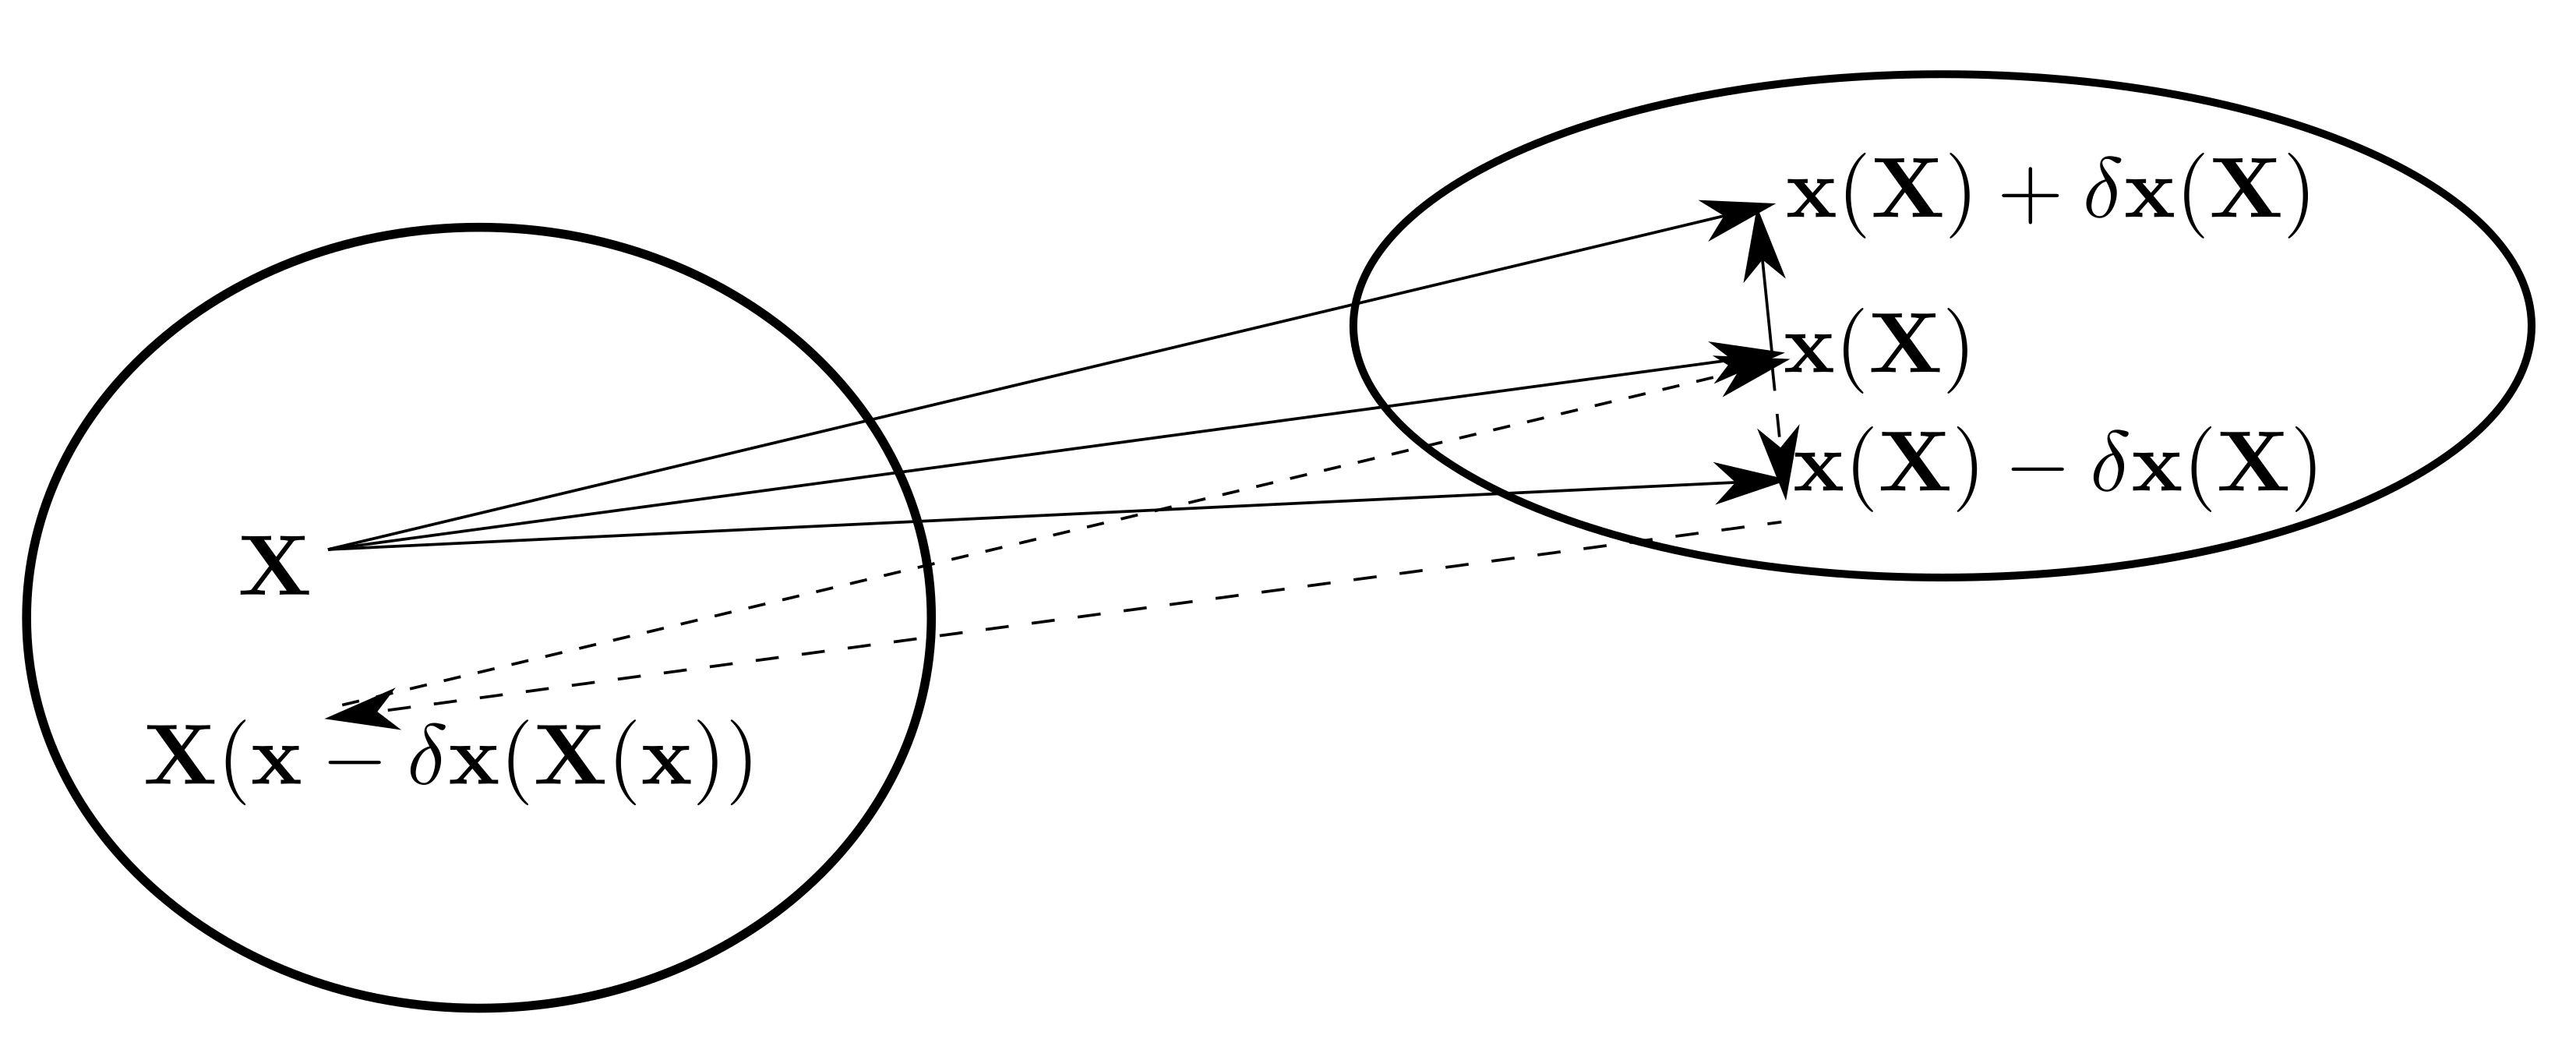
\includegraphics[scale=0.3]{trafo.png}
    \caption{Demonstration of formula \eqref{eq.xX} (the dashed triangle). The left manifold represents the Lagrangian configuration while right represents the Eulerian configuration. }
    \label{fig.trafo}
\end{figure}

The functional derivatives of the Eulerian fields with respect to the Lagrangian fields are necessary to perform the projection. Let us start with the Lagrangian density in the Eulerian frame, $\rho_0(\xx)\stackrel{def}{=}\rho_0(\XX(\xx))$. This slightly overloaded notation is used throughout this appendix. To avoid confusion, the spatial variables on which the fields depend will be always indicated. To find functional derivative of $\rho_0(\xx)$ with respect to $\xx(\XX)$ we study 
\begin{equation}
	\rho_0(\xx;\xx+\delta\xx)\stackrel{def}{=} \rho_0(\XX(\xx)+\delta\XX(\xx)),
\end{equation}
where $\delta\XX(\xx)$ is the perturbation of mapping $\XX(\xx)$ induced by perturbation $\delta\xx(\XX)$. Using relation \eqref{eq.xX}, we obtain 
\begin{eqnarray}
	\rho_0(\xx;\xx+\delta\xx) &=& \rho_0(\XX(\xx-\delta\xx(\XX(\xx)))) = \rho_0(\xx-\delta\xx(\XX(\xx)))\nonumber\\
	&=&\rho_0(\xx)-\partial_k \rho_0(\xx) \delta x^k(\XX(\xx))+\OBig(\delta\xx)^2\nonumber\\
	&=&\rho_0(\xx)+\int\dX \left(-\partial_k \rho_0(\xx) \delta(\XX-\XX(\xx))\right)\delta x^k(\XX)+\OBig(\delta\xx)^2,
\end{eqnarray}
which means that
\begin{equation}\label{eq.rho0x}
	\frac{\delta \rho_0(\xx)}{\delta x^k(\XX)} = -\partial_k \rho_0(\xx) \delta(\XX-\XX(\xx)).
\end{equation}

\subsection{Derivative of the Eulerian deformation gradient $\FF(\xx)$}
The Eulerian mass density $\rho(\xx)$ is equal to $\rho_0(\xx)$ multiplied by Jacobian of the mapping $\XX(\xx)$, and so to acquire the functional derivative of $\rho(\xx)$ we have to first  deal with functional derivative of the Eulerian deformation gradient
\begin{equation}
	\FF(\xx)\stackrel{def}{=}\frac{\partial \xx}{\partial \XX}\Big|_{\XX(\xx)}.
\end{equation}
Using again relation \eqref{eq.xX} we have
\begin{eqnarray}
	\F{i}{I}(\xx;\xx+\delta\xx) &\stackrel{def}{=}&\frac{\partial x^i(\XX) +\delta 
	x^i(\XX)}{\partial X^I}\Big|_{\XX(\xx-\delta\xx(\XX(\xx)))}\\
	&=&\frac{\partial x^i}{\partial X^I}\Big|_{\XX(\xx-\delta\xx(\XX(\xx)))} + \frac{\partial \delta x^i}{\partial X^I}\Big|_{\XX(\xx)}+\OBig(\delta\xx)^2\nonumber\\
	&=&\int\dX\delta(\XX-\XX(\xx)) \frac{\partial \delta x^i}{\delta X^I} 
	+\underbrace{\frac{\partial x^i}{\partial X^I}\Big|_{\XX(\xx)}}_{=\F{i}{I}(\xx)} -\partial_k 
	\F{i}{I}(\xx)\delta x^k(\XX(\xx)) + \OBig(\delta\xx)^2\nonumber\\
	&=&\F{i}{I}(\xx) - \int\dX\frac{\partial \delta(\XX-\XX(\xx))}{\partial X^I}\delta x^i(\XX) 
	-\int\dX\partial_k \F{i}{I}(\xx)\delta(\XX-\XX(\xx))\delta x^k(\XX),\nonumber
\end{eqnarray}
which means that the sought functional derivative reads
\begin{equation}
	\frac{\delta \F{i}{I}(\xx)}{\delta x^k(\XX)} = 
	- \frac{\partial \delta(\XX-\XX(\xx))}{\partial X^I}\delta^i_k -\partial_k 
	\F{i}{I}(\xx)\delta(\XX-\XX(\xx)).
\end{equation}

\subsection{Derivative of the Eulerian mass density $\rho(\xx)$}
Now we can finish the calculation of the functional derivative of the Eulerian density $\rho(\xx)$ with respect to $\xx(\XX)$. The first part, derivative of $\rho_0(\xx)$, has already been obtained before in Eq. \eqref{eq.rho0x}. What remains is to calculate derivative of determinant $\det \FF(\xx)$ with respect to $\xx(\XX)$. 

Considering determinant of a general matrix $\CC$, its variation when the matrix is perturbed by $\delta\CC$ reads
\begin{equation}
	\det(\CC+\delta\CC) = \det(\CC)\cdot\det(\Id+\CC^{-1}\cdot\delta\CC) = \det\CC\cdot\Tr(\CC^{-1}\cdot\delta\CC) + \OBig(\delta \CC)^2.
\end{equation}
Therefore, derivative of $\det(\FF)$ is
\begin{equation}
	\frac{\delta \det \FF^{-1}(\xx)}{\delta x^k(\XX)}
	= -\frac{1}{(\det \FF(\xx))^2} \det \FF(\xx) \frac{\partial X^I}{\partial x^i} \frac{\delta 
	\F{i}{I}(\xx)}{\delta x^k(\XX)}.
\end{equation}

Derivative of the Eulerian density finally reads
\begin{eqnarray}
	\frac{\delta \rho(\xx)}{\delta x^k(\XX)}&=&\frac{\delta \rho_0(\xx)}{\delta x^k(\XX)} \det \frac{\partial \XX}{\partial \xx}
	-\frac{\rho_0(\xx)}{(\det \FF(\xx))^2} \det \FF(\xx) \frac{\partial X^I}{\partial x^i} 
	\frac{\delta \F{i}{I}(\xx)}{\delta x^k(\XX)}\nonumber\\
	&=&-\partial_k \rho_0(\xx) \delta(\XX-\XX(\xx))\frac{1}{\det\FF(\xx)}\nonumber\\
	&&
	+\frac{\rho_0(\xx)}{\det \FF(\xx)} \frac{\partial X^I}{\partial x^i} \frac{\partial \delta(\XX-\XX(\xx))}{\partial X^I}\delta^i_k \nonumber\\
	&&+\frac{\rho_0(\xx)}{\det \FF(\xx)} \frac{\partial X^I}{\partial x^i} \partial_k 
	\F{i}{I}(\xx)\delta(\XX-\XX(\xx)).
\end{eqnarray}

\subsection{Derivative of the Eulerian entropy density $s(\xx)$}
Having calculated derivative of mass density, the result for entropy density $s(\xx)=s_0(\xx)/\det\FF(\xx)$  is analogous,
\begin{eqnarray}
	\frac{\delta s(\xx)}{\delta x^k(\XX)}&=&
	-\partial_k s_0(\xx) \delta(\XX-\XX(\xx))\frac{1}{\det\FF(\xx)}\nonumber\\
	&&
	+\frac{s_0(\xx)}{\det \FF(\xx)} \frac{\partial X^I}{\partial x^i} \frac{\partial \delta(\XX-\XX(\xx))}{\partial X^I}\delta^i_k \nonumber\\
	&&+\frac{s_0(\xx)}{\det \FF(\xx)} \frac{\partial X^I}{\partial x^i} \partial_k 
	\F{i}{I}(\xx)\delta(\XX-\XX(\xx)).
\end{eqnarray}

\subsection{Derivative of the Eulerian momentum density $\mm(\xx)$}
The functional derivative of $\mm(\xx)=\MM(\XX(\xx))/\det \FF(\xx)$ with respect to $\xx(\XX)$ has the same form as derivatives of $\rho(\xx)$ and $s(\xx)$,
\begin{eqnarray}
	\frac{\delta m_l(\xx)}{\delta x^k(\XX)}&=&
	-\partial_k M_l(\xx) \delta(\XX-\XX(\xx))\frac{1}{\det\FF(\xx)}\nonumber\\
	&&
	+\frac{M_l(\xx)}{\det \FF(\xx)} \frac{\partial X^I}{\partial x^i} \frac{\partial \delta(\XX-\XX(\xx))}{\partial X^I}\delta^i_k \nonumber\\
	&&+\frac{M_l(\xx)}{\det \FF(\xx)} \frac{\partial X^I}{\partial x^i} \partial_k 
	\F{i}{I}(\xx)\delta(\XX-\XX(\xx)).
\end{eqnarray}

But the field $\mm(\xx)$ also depends on the yet unused Lagrangian field $\MM(\XX)$. Derivative with respect to this fields is
\begin{eqnarray}\label{eq.mM}
	\frac{\delta m_l(\xx)}{\delta M_k(\XX)} = \delta^k_l \frac{\delta(\XX-\XX(\xx))}{\det\FF(\xx)},
\end{eqnarray}
as follows from the formulas 
\begin{equation}
    \MM(\XX(\xx)) = \int\dX \delta(\XX-\XX(\xx)) \MM(\XX)
\end{equation}
and
\begin{equation}
    \frac{\delta M_k(\XX(\xx)}{\delta M_l(\XX)} = \delta^l_k \delta(\XX-\XX(\xx)).
\end{equation}

\subsection{Derivative of an arbitrary Eulerian functional}
Derivative of an arbitrary smooth enough functional\footnote{Functionals $F$ and $G$ are not used here to avoid confusing with tensor $\FF$.} of the Eulerian fields $C(\rho(\xx), \mm(\xx), s(\xx), \FF(\xx))$ with respect to the Lagrangian field $\xx(\XX)$ can be calculated by chain rule as
\begin{equation}\label{eq.Cx}
	\frac{\delta C}{\delta x^k(\XX)} = \int\dx \left(\frac{\delta C}{\delta \rho(\xx)}\frac{\delta \rho(\xx)}{\delta x^k(\XX)}
	+\frac{\delta C}{\delta m_l(\xx)}\frac{\delta m_l(\xx)}{\delta x^k(\XX)}
	+\frac{\delta C}{\delta s(\xx)}\frac{\delta s(\xx)}{\delta x^k(\XX)}
	+\frac{\delta C}{\delta \F{i}{I}(\xx)}\frac{\delta \F{i}{I}(\xx)}{\delta x^k(\XX)}\right).
\end{equation}
Similarly derivative of an arbitrary functional $D(\rho(\xx), \mm(\xx), s(\xx), \FF(\xx))$ with respect to the Lagrangian $\MM(\XX)$ field is
\begin{equation}
	\frac{\delta D}{\delta M_k(\XX)} = \int\dx \frac{\delta D}{\delta m_l(\xx)}\frac{\delta m_l(\xx)}{\delta M_k(\XX)},
\end{equation}
which, using Eq. \eqref{eq.mM}, can be rewritten more explicitly as
\begin{eqnarray}
	\frac{\delta D}{\delta M_k(\XX)} &=& \int\dx \frac{\delta D}{\delta m_l(\xx)}\delta^k_l \frac{\delta(\XX-\XX(\xx))}{\det\FF(\xx)}\nonumber\\
	&=& \int\dx \frac{\delta D}{\delta m_k(\xx)}\delta(\XX-\XX(\xx))\det\frac{\partial \XX}{\partial \xx}.
\end{eqnarray}
The $\delta-$distribution can be seen as the limit of a sequence of smooth functions (e.g. Gaussians), $f_n(\xx)\stackrel{\mathcal{D}'}{\to}\delta(\xx)$. Therefore, the last integral can be rewritten as
\begin{eqnarray}
	\frac{\delta D}{\delta M_k(\XX)} &=& \lim_{n\to\infty}\int\dx \frac{\delta D}{\delta m_k(\xx)}f_n(\XX-\XX(\xx)) \det\frac{\partial \XX}{\partial \xx}\nonumber\\
	&=& \lim_{n\to\infty}\int\dX' \frac{\delta D}{\delta m_k(\xx)}\Big|_{\xx(\XX')} f_n(\XX-\XX(\xx(\XX'))) \nonumber\\
	&=& \int\dX' \frac{\delta D}{\delta m_k(\xx)}\Big|_{\xx(\XX')} \lim_{n\to\infty}f_n(\XX-\XX') 
	= \int\dX' \frac{\delta D}{\delta m_k(\xx)}\Big|_{\xx(\XX')} \delta(\XX-\XX') \nonumber\\
	&=&\frac{\delta D}{\delta m_k(\xx)}\Big|_{\xx(\XX)}.
\end{eqnarray}
Now we are finally in position to calculate the Lagrangian Poisson bracket Eq. \eqref{eq.PB.L} for the Eulerian functionals $C$ and $D$. 

\subsection{The Eulerian Poisson bracket}
Bracket \eqref{eq.PB.L} is the sum of terms like
\begin{equation}
	\int\dX \frac{\delta C}{\delta x^k(\XX)} \frac{\delta D}{\delta M_k(\XX)},
\end{equation}
where the former functional derivative consists of all terms in Eq. \eqref{eq.Cx}. Let us first take only the term with derivative $C_{\rho(\xx)}$,
\begin{eqnarray}
	\int\dX \int\dx \frac{\delta C}{\delta \rho(\xx)}&&
	\left[
		-\partial_k \rho_0(\xx) \delta(\XX-\XX(\xx))\frac{1}{\det\FF(\xx)}\right.\nonumber\\
	&&
	+\frac{\rho_0(\xx)}{\det \FF(\xx)} \frac{\partial X^I}{\partial x^i} \frac{\partial \delta(\XX-\XX(\xx))}{\partial X^I}\delta^i_k \nonumber\\
	&&\left.+\frac{\rho_0(\xx)}{\det \FF(\xx)} \frac{\partial X^I}{\partial x^i} \partial_k 
	\F{i}{I}(\xx)\delta(\XX-\XX(\xx))\right]
\frac{\delta D}{\delta m_k(\xx)}\Big|_{\xx(\XX)}\nonumber\\
	&=& \int\dx \frac{\delta C}{\delta \rho(\xx)}\left[
		-\partial_k \rho_0(\xx)\det\FF^{-1}(\xx)\frac{\delta D}{\delta m_k(\xx)} \right.\nonumber\\
		&&-\rho_0(\xx) \partial_k \det \FF^{-1}(\xx)\frac{\delta D}{\delta m_k(\xx)} \nonumber\\
		&&\left.-\frac{\rho_0(\xx)}{\det \FF(\xx)} \frac{\partial X^I}{\partial x^i} \int\dX \delta(\XX-\XX(\xx))\frac{\partial}{\partial X^I}\frac{\delta D}{\delta m_i(\xx)}\Big|_{\xx(\XX)}\right]\nonumber\\
	&=&\int\dx \frac{\delta C}{\delta \rho(\xx)}\left[-\partial_k \rho(\xx)\frac{\delta D}{\delta m_k(\xx)}\right.\nonumber\\
	&&\left.\qquad -\rho(\xx) \partial_i \frac{\delta D}{\delta m_i(\xx)}\right]\nonumber\\
	&=& \int\dx \rho(\xx)\partial_i \frac{\delta C}{\delta \rho(\xx)} \frac{\delta D}{\delta m_i(\xx)},
\end{eqnarray}
which is obviously a part of the final Eulerian Poisson bracket \eqref{eq.PB.Eu}. In the same fashion we obtain
\begin{equation}
	\int\dX \int\dx \frac{\delta C}{\delta m_l(\xx)} \frac{\delta m_l(\xx)}{\delta x^k(\XX)} \frac{\delta D}{\delta M_k(\XX)}
	= \int\dx m_i(\xx)\partial_j \frac{\delta C}{\delta m_i(\xx)} \frac{\delta D}{\delta m_j(\xx)}
\end{equation}
and
\begin{equation}
	\int\dX \int\dx \frac{\delta C}{\delta s(\xx)} \frac{\delta s(\xx)}{\delta x^k(\XX)} \frac{\delta D}{\delta M_k(\XX)}
	= \int\dx s(\xx)\partial_j \frac{\delta C}{\delta s(\xx)} \frac{\delta D}{\delta m_j(\xx)}.
\end{equation}
So far we have recovered the $\{C,D\}^{(FM)}$ part of the bracket (the antisymmetric part is obtained as negative of the same terms with $C$ and $D$ swapped).

The part dependent on the Eulerian deformation gradient $\FF(\xx)$ is calculated similarly as follows.
\begin{align}
	&\int\dX \int\dx \frac{\delta C}{\delta \F{i}{I}(\xx)} \frac{\delta \F{i}{I}(\xx)}{\delta 
	x^k(\XX)} \frac{\delta D}{\delta M_k(\XX)}\nonumber\\
	&\qquad=\int\dX \int\dx \frac{\delta C}{\delta \F{i}{I}(\xx)}\left[
	- \frac{\partial \delta(\XX-\XX(\xx))}{\partial X^I}\delta^i_k
	-\partial_k \F{i}{I}(\xx)\delta(\XX-\XX(\xx))\right]\frac{\delta D}{\delta 
	m_k(\xx)}\Big|_{\xx(\XX)}\nonumber\\
&\qquad=\int\dx  \frac{\delta C}{\delta \F{i}{I}(\xx)}\left[
	\int\dX \delta(\XX-\XX(\xx)) \frac{\partial}{\partial X^I}\frac{\delta D}{\delta m_i(\xx)}\Big|_{\xx(\XX)}
	-\partial_k \F{i}{I}(\xx)\frac{\delta D}{\delta m_k(\xx)}\right]\nonumber\\
&\qquad=\int\dx  \frac{\delta C}{\delta \F{i}{I}(\xx)}\left[
	\frac{\partial x^j}{\partial X^I}\Big|_{\XX(\xx)}\frac{\partial}{\partial x^j}\frac{\delta D}{\delta m_i(\xx)}
	-\partial_k \F{i}{I}(\xx)\frac{\delta D}{\delta m_k(\xx)}\right]\nonumber\\
&\qquad=\int\dx  \frac{\delta C}{\delta \F{i}{I}(\xx)}\left(\F{j}{I}(\xx)\partial_j \frac{\delta 
D}{\delta m_i(\xx)}
	-\partial_k \F{i}{I}(\xx)\frac{\delta D}{\delta m_k(\xx)}\right),
\end{align}
which is the remaining part of bracket \eqref{eq.PB.Eu}. 

In summary, Eulerian Poisson bracket \eqref{eq.PB.Eu}, which expresses kinematics of fields $\rho(\xx)$, $\mm(\xx)$, $s(\xx)$ and $\FF(\xx)$, has been derived by projection from the Lagrangian canonical Poisson bracket \eqref{eq.PB.L}, expressing kinematics of $\xx(\XX)$ and $\MM(\XX)$.



\section{From deformation gradient to the Left Cauchy-Green tensor}\label{sec.F-B}
Derivative of the left Cauchy-Green tensor $\BB(\xx)$ with respect to the Eulerian deformation gradient is
\begin{equation}
	\frac{\partial B^{ij}(\xx)}{\partial \F{k}{K}} = \delta^{\sI\sJ}(\delta^i_{\ k} \delta^\sK_\sI 
	\F{j}{J} +  
	\F{i}{I} \delta^j_{\ k} \delta^\sK_\sJ)
	= \delta^{\sK\sJ}\delta^i_k \F{j}{J} +  \delta^{\sI\sK} \F{i}{I} \delta^j_k.
\end{equation}
Derivative of a functional $C(\FF)$ then becomes
\begin{equation}
	\frac{\delta C}{\delta \F{k}{K}(\xx)} = 
	\frac{\delta C}{\delta B^{kj}(\xx)}\delta^{\sK\sJ} \F{j}{J} +  \frac{\delta C}{\delta 
	B^{ik}(\xx)}\delta^{\sI\sK} \F{i}{I},
\end{equation}
and after plugging this relation into bracket \eqref{eq.PB.Eu} we obtain bracket \eqref{eq.PB.B} easily.


\section{From deformation gradient to distortion}\label{sec.F-A}
The purpose of this section is to show more details on the projection from bracket \eqref{eq.PB.Eu} to bracket \eqref{eq.PB.A}, expressing kinematics of distortion. The distortion is the inverse of the Eulerian deformation gradeint $\FF(\xx)$, 
\begin{equation}
	\A{I}{i}(\xx) \F{j}{I}(\xx) = \delta^j_{\ i}.
\end{equation}
Taking derivative of this equality with respect to $\F{k}{K}(\xx)$ leads to
\begin{equation}
	\frac{\partial \A{I}{i}}{\partial \F{k}{K}} \F{j}{I} = -\A{K}{i} \delta^j_{\ k}.
\end{equation}
After multiplication by $\A{J}{j}$ we obtain
\begin{equation}\label{app.eq.dAdF}
	\frac{\partial \A{L}{l}}{\partial \F{j}{J}} = -\A{J}{l} \A{L}{j},
\end{equation}
from which it follows that 
\begin{equation}
	\frac{\delta C}{\delta \F{j}{J}} = \frac{\delta C}{\delta \A{L}{l}(\xx)} \frac{\partial 
	\A{L}{l}}{\partial \F{j}{J}} = -\frac{\delta C}{\delta \A{L}{l}} \A{J}{l} \A{L}{j}
\end{equation}
for arbitrary functional $C(\FF)$.

Plugging this last relation into bracket \eqref{eq.PB.Eu} immediatly leads to bracket \eqref{eq.PB.A}.


\end{document}
